\chapter{Deep Graph Networks} \label{ch:dgn}

The \gls{rnn} and \gls{recnn} models presented in Chapter \ref{ch:deep-learning-structures} share the idea that the state transition function is applied locally and recursively on the structure to compute the state vectors. Extending it to arbitrary graphs (which can have cycles) would require to apply the state transition function recursively to the neighbors of a vertex. However, this approach is not applicable to general graphs. In fact, the presence of cycles creates \emph{mutual dependencies}, which are difficult to model recursively and may lead to infinite loops when computing the states of vertices in parallel. While this issue can be overcome by resorting to canonization techniques that provide an ordering between the vertices, it is not feasible in many practical cases. \glspl{dgn} are a class of \glspl{nn} which can process arbitrary graphs, even in presence of cycles. The solution adopted by \glspl{dgn} to the problem of modelling mutual dependencies is to update the state of the vertices according to an \emph{iterative} scheme. Specifically, the hidden state of a vertex is updated as a function of the hidden state of the same vertex at the previous iteration. Given an attributed graph $\GraphU{g}$ with vertex features $\GraphFeatures{x}{g} = \Set{\Elem{x}{v} \mid v \in \Nodes{g}}$, the state transition function computed by a \gls{dgn}, applied locally to each vertex of $v \in \Nodes{g}$, has the following form:
\begin{align*}
    \StateVector{v}{\ell}=
    \begin{cases}
        \Elem{x}{v} & \mathrm{if}\; \ell = 0\\
        \EncTrans^{(\ell)}(\Elem{x}{v}, \StateVector{v}{\ell-1}) & \mathrm{otherwise},
    \end{cases}
\end{align*}
where $\StateVector{v}{\ell} \in \Real^h$ is now the state of vertex $v$ at iteration $\ell$, and $\EncTrans = \EncTrans^{1} \circ \EncTrans^{2} \circ \ldots \circ \EncTrans^{(\ell)}$. Notice how the value of the state vector does not depend on the value of the neighboring state vectors, but to the same state vector at the previous iteration. Following, we slightly change terminology and refer to the vertices of a graph as nodes, in accordance to the terminology currently used in the literature. For the same reason, we shall use the following terminology as regards the supervised tasks that can be learned with \glspl{dgn}:
\begin{itemize}
    \item structure-to-structure tasks shall now be termed \keyword{node classification} tasks if the targets are discrete node labels, or \keyword{node regression} tasks if the targets associated to the nodes are continuous vectors or scalars. We further distinguish among \emph{inductive} node classification (respectively, regression) tasks, if the prediction concerns unseen graphs; and \emph{transductive} node classification (respectively, regression) tasks, if the structure of the graph is fixed (\ie, the dataset is composed of one single graph), and the task is to predict from a subset of nodes for whose target is not known. The transductive setting is often referred to as semi-supervised node classification (respectively, regression);
    \item structure-to-element tasks shall now be termed \keyword{graph classification} tasks if the target associated to the graph is a discrete label, or \keyword{graph regression} tasks if the targets are continuous vectors (or scalars).
\end{itemize}

\section{Contextual Processing of Graph Information}
Besides solving the problem of mutual dependencies in the state computations, the iterative scheme has another important purpose, that of propagating the local information of a node to the other nodes of the graph. This process is known under several names, such as \keyword{context diffusion}. Informally, the context of a node is the set of nodes that directly or indirectly contribute to determine its hidden state; for a more formal characterization of the context, see \citep{micheli2009nn4g}. Context diffusion in a graph is obtained through \keyword{message passing}, \ie by repeatedly applying the following procedures:
\begin{itemize}
    \item each node constructs a \emph{message} vector using its hidden state, which is sent to the immediate neighbors according to the graph structure;
    \item each node receives messages from its neighbors, which are used to update its current hidden state through the state transition function.
\end{itemize}
Message passing is bootstrapped by initializing the hidden state of the nodes appropriately, so that an initial message can be created. Usually, this initial message is the vector of node features. Using the example graph of Figure \ref{fig:context-diffusion} as reference, we now explain how the context flows through the nodes as message passing is iterated. At iteration $\ell=2$, the vertex $v$ receives a single message from its only neighbor, $u$. The incoming message was constructed using information about the state of $u$ at $\ell=1$, which in turn was obtained through the state of neighbors of $u$ at $\ell=0$ (including $v$ itself). Thus, the context of $v$ at iteration $\ell=2$ includes $u$ as well as the neighbors of $u$. It is clear that, for this particular case, at iteration $\ell=3$ the context of $v$ would include all the nodes in the graph. Clearly, by iterating message passing, the nodes are able to acquire information from other nodes farther away in the graph.
\begin{figure*}[h!]
    \centering
    \resizebox{.8\textwidth}{!}{

\tikzset{every picture/.style={line width=0.75pt}} %set default line width to 0.75pt        

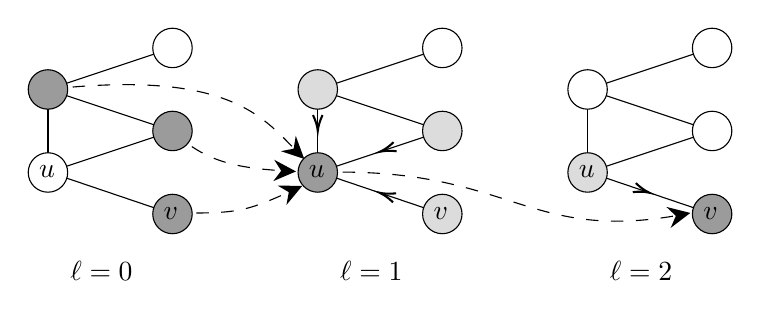
\begin{tikzpicture}[x=0.75pt,y=0.75pt,yscale=-1,xscale=1]
%uncomment if require: \path (0,160); %set diagram left start at 0, and has height of 160

%Curve Lines [id:da4313717085077018] 
\draw  [dash pattern={on 4.5pt off 4.5pt}]  (40.5,40.5) .. controls (128.99,30.61) and (144.66,54.47) .. (162.09,72.11) ;
\draw [shift={(164,74)}, rotate = 224.13] [fill={rgb, 255:red, 0; green, 0; blue, 0 }  ][line width=0.08]  [draw opacity=0] (10.72,-5.15) -- (0,0) -- (10.72,5.15) -- (7.12,0) -- cycle    ;
%Curve Lines [id:da6954216550236572] 
\draw  [dash pattern={on 4.5pt off 4.5pt}]  (100.5,60.5) .. controls (116.13,75.22) and (130.65,78.52) .. (157.08,79.86) ;
\draw [shift={(160,80)}, rotate = 182.53] [fill={rgb, 255:red, 0; green, 0; blue, 0 }  ][line width=0.08]  [draw opacity=0] (10.72,-5.15) -- (0,0) -- (10.72,5.15) -- (7.12,0) -- cycle    ;
%Curve Lines [id:da3347980352129689] 
\draw  [dash pattern={on 4.5pt off 4.5pt}]  (100,100) .. controls (132.69,100.24) and (135.08,99.78) .. (160.57,88.11) ;
\draw [shift={(163,87)}, rotate = 515.36] [fill={rgb, 255:red, 0; green, 0; blue, 0 }  ][line width=0.08]  [draw opacity=0] (10.72,-5.15) -- (0,0) -- (10.72,5.15) -- (7.12,0) -- cycle    ;
%Curve Lines [id:da07095702036161233] 
\draw  [dash pattern={on 4.5pt off 4.5pt}]  (170.5,80.5) .. controls (264.25,77.28) and (270.58,115.47) .. (347.64,100.47) ;
\draw [shift={(350,100)}, rotate = 528.4200000000001] [fill={rgb, 255:red, 0; green, 0; blue, 0 }  ][line width=0.08]  [draw opacity=0] (10.72,-5.15) -- (0,0) -- (10.72,5.15) -- (7.12,0) -- cycle    ;
%Straight Lines [id:da47912352597118213] 
\draw    (40.5,50) -- (40.5,71) ;
%Straight Lines [id:da9922159879153771] 
\draw    (40.5,40.5) -- (100.5,60.5) ;
%Straight Lines [id:da20693867709022928] 
\draw    (40.5,80.5) -- (100.5,60.5) ;
%Straight Lines [id:da12726884670105187] 
\draw    (40,80) -- (100.5,100.5) ;
%Straight Lines [id:da005529487369804631] 
\draw    (100.5,20.5) -- (40.5,40.5) ;
%Shape: Circle [id:dp12978240920475836] 
\draw  [fill={rgb, 255:red, 155; green, 155; blue, 155 }  ,fill opacity=1 ] (31,40.5) .. controls (31,35.25) and (35.25,31) .. (40.5,31) .. controls (45.75,31) and (50,35.25) .. (50,40.5) .. controls (50,45.75) and (45.75,50) .. (40.5,50) .. controls (35.25,50) and (31,45.75) .. (31,40.5) -- cycle ;
%Shape: Circle [id:dp44461896764010267] 
\draw  [fill={rgb, 255:red, 255; green, 255; blue, 255 }  ,fill opacity=1 ] (91,20.5) .. controls (91,15.25) and (95.25,11) .. (100.5,11) .. controls (105.75,11) and (110,15.25) .. (110,20.5) .. controls (110,25.75) and (105.75,30) .. (100.5,30) .. controls (95.25,30) and (91,25.75) .. (91,20.5) -- cycle ;
%Shape: Circle [id:dp8226342601300562] 
\draw  [fill={rgb, 255:red, 155; green, 155; blue, 155 }  ,fill opacity=1 ] (91,60.5) .. controls (91,55.25) and (95.25,51) .. (100.5,51) .. controls (105.75,51) and (110,55.25) .. (110,60.5) .. controls (110,65.75) and (105.75,70) .. (100.5,70) .. controls (95.25,70) and (91,65.75) .. (91,60.5) -- cycle ;
%Shape: Circle [id:dp9576590983310105] 
\draw  [fill={rgb, 255:red, 255; green, 255; blue, 255 }  ,fill opacity=1 ] (31,80.5) .. controls (31,75.25) and (35.25,71) .. (40.5,71) .. controls (45.75,71) and (50,75.25) .. (50,80.5) .. controls (50,85.75) and (45.75,90) .. (40.5,90) .. controls (35.25,90) and (31,85.75) .. (31,80.5) -- cycle ;
%Shape: Circle [id:dp6767076773328078] 
\draw  [fill={rgb, 255:red, 155; green, 155; blue, 155 }  ,fill opacity=1 ] (91,100.5) .. controls (91,95.25) and (95.25,91) .. (100.5,91) .. controls (105.75,91) and (110,95.25) .. (110,100.5) .. controls (110,105.75) and (105.75,110) .. (100.5,110) .. controls (95.25,110) and (91,105.75) .. (91,100.5) -- cycle ;
%Straight Lines [id:da3797310936600804] 
\draw    (170.5,50) -- (170.5,71) ;
\draw [shift={(170.5,60.5)}, rotate = 270] [color={rgb, 255:red, 0; green, 0; blue, 0 }  ][line width=0.75]    (7.65,-2.3) .. controls (4.86,-0.97) and (2.31,-0.21) .. (0,0) .. controls (2.31,0.21) and (4.86,0.98) .. (7.65,2.3)   ;
%Straight Lines [id:da39313117597338243] 
\draw    (170.5,40.5) -- (230.5,60.5) ;
%Straight Lines [id:da11909283508234703] 
\draw    (170.5,80.5) -- (230.5,60.5) ;
\draw [shift={(200.5,70.5)}, rotate = 341.57] [color={rgb, 255:red, 0; green, 0; blue, 0 }  ][line width=0.75]    (7.65,-2.3) .. controls (4.86,-0.97) and (2.31,-0.21) .. (0,0) .. controls (2.31,0.21) and (4.86,0.98) .. (7.65,2.3)   ;
%Straight Lines [id:da3511148855222339] 
\draw    (170,80) -- (230.5,100.5) ;
\draw [shift={(200.25,90.25)}, rotate = 18.72] [color={rgb, 255:red, 0; green, 0; blue, 0 }  ][line width=0.75]    (7.65,-2.3) .. controls (4.86,-0.97) and (2.31,-0.21) .. (0,0) .. controls (2.31,0.21) and (4.86,0.98) .. (7.65,2.3)   ;
%Straight Lines [id:da6106293032869707] 
\draw    (230.5,20.5) -- (170.5,40.5) ;
%Shape: Circle [id:dp4701031138690044] 
\draw  [fill={rgb, 255:red, 220; green, 220; blue, 220 }  ,fill opacity=1 ] (161,40.5) .. controls (161,35.25) and (165.25,31) .. (170.5,31) .. controls (175.75,31) and (180,35.25) .. (180,40.5) .. controls (180,45.75) and (175.75,50) .. (170.5,50) .. controls (165.25,50) and (161,45.75) .. (161,40.5) -- cycle ;
%Shape: Circle [id:dp5321807173132955] 
\draw  [fill={rgb, 255:red, 255; green, 255; blue, 255 }  ,fill opacity=1 ] (221,20.5) .. controls (221,15.25) and (225.25,11) .. (230.5,11) .. controls (235.75,11) and (240,15.25) .. (240,20.5) .. controls (240,25.75) and (235.75,30) .. (230.5,30) .. controls (225.25,30) and (221,25.75) .. (221,20.5) -- cycle ;
%Shape: Circle [id:dp554517566024453] 
\draw  [fill={rgb, 255:red, 220; green, 220; blue, 220 }  ,fill opacity=1 ] (221,60.5) .. controls (221,55.25) and (225.25,51) .. (230.5,51) .. controls (235.75,51) and (240,55.25) .. (240,60.5) .. controls (240,65.75) and (235.75,70) .. (230.5,70) .. controls (225.25,70) and (221,65.75) .. (221,60.5) -- cycle ;
%Shape: Circle [id:dp6234497550508977] 
\draw  [fill={rgb, 255:red, 155; green, 155; blue, 155 }  ,fill opacity=1 ] (161,80.5) .. controls (161,75.25) and (165.25,71) .. (170.5,71) .. controls (175.75,71) and (180,75.25) .. (180,80.5) .. controls (180,85.75) and (175.75,90) .. (170.5,90) .. controls (165.25,90) and (161,85.75) .. (161,80.5) -- cycle ;
%Shape: Circle [id:dp6481128593514689] 
\draw  [fill={rgb, 255:red, 220; green, 220; blue, 220 }  ,fill opacity=1 ] (221,100.5) .. controls (221,95.25) and (225.25,91) .. (230.5,91) .. controls (235.75,91) and (240,95.25) .. (240,100.5) .. controls (240,105.75) and (235.75,110) .. (230.5,110) .. controls (225.25,110) and (221,105.75) .. (221,100.5) -- cycle ;
%Straight Lines [id:da010045754906601312] 
\draw    (300.5,50) -- (300.5,71) ;
%Straight Lines [id:da9723039406561984] 
\draw    (300.5,40.5) -- (360.5,60.5) ;
%Straight Lines [id:da7207693173524592] 
\draw    (300.5,80.5) -- (360.5,60.5) ;
%Straight Lines [id:da047867810436508895] 
\draw    (300,80) -- (360.5,100.5) ;
\draw [shift={(330.25,90.25)}, rotate = 198.72] [color={rgb, 255:red, 0; green, 0; blue, 0 }  ][line width=0.75]    (7.65,-2.3) .. controls (4.86,-0.97) and (2.31,-0.21) .. (0,0) .. controls (2.31,0.21) and (4.86,0.98) .. (7.65,2.3)   ;
%Straight Lines [id:da13877434621766804] 
\draw    (360.5,20.5) -- (300.5,40.5) ;
%Shape: Circle [id:dp9753163859311793] 
\draw  [fill={rgb, 255:red, 255; green, 255; blue, 255 }  ,fill opacity=1 ] (291,40.5) .. controls (291,35.25) and (295.25,31) .. (300.5,31) .. controls (305.75,31) and (310,35.25) .. (310,40.5) .. controls (310,45.75) and (305.75,50) .. (300.5,50) .. controls (295.25,50) and (291,45.75) .. (291,40.5) -- cycle ;
%Shape: Circle [id:dp03916750111680778] 
\draw  [fill={rgb, 255:red, 255; green, 255; blue, 255 }  ,fill opacity=1 ] (351,20.5) .. controls (351,15.25) and (355.25,11) .. (360.5,11) .. controls (365.75,11) and (370,15.25) .. (370,20.5) .. controls (370,25.75) and (365.75,30) .. (360.5,30) .. controls (355.25,30) and (351,25.75) .. (351,20.5) -- cycle ;
%Shape: Circle [id:dp7074039311567142] 
\draw  [fill={rgb, 255:red, 255; green, 255; blue, 255 }  ,fill opacity=1 ] (351,60.5) .. controls (351,55.25) and (355.25,51) .. (360.5,51) .. controls (365.75,51) and (370,55.25) .. (370,60.5) .. controls (370,65.75) and (365.75,70) .. (360.5,70) .. controls (355.25,70) and (351,65.75) .. (351,60.5) -- cycle ;
%Shape: Circle [id:dp4904701423686293] 
\draw  [fill={rgb, 255:red, 220; green, 220; blue, 220 }  ,fill opacity=1 ] (291,80.5) .. controls (291,75.25) and (295.25,71) .. (300.5,71) .. controls (305.75,71) and (310,75.25) .. (310,80.5) .. controls (310,85.75) and (305.75,90) .. (300.5,90) .. controls (295.25,90) and (291,85.75) .. (291,80.5) -- cycle ;
%Shape: Circle [id:dp8890572986824241] 
\draw  [fill={rgb, 255:red, 155; green, 155; blue, 155 }  ,fill opacity=1 ] (351,100.5) .. controls (351,95.25) and (355.25,91) .. (360.5,91) .. controls (365.75,91) and (370,95.25) .. (370,100.5) .. controls (370,105.75) and (365.75,110) .. (360.5,110) .. controls (355.25,110) and (351,105.75) .. (351,100.5) -- cycle ;

% Text Node
\draw (355,96) node [anchor=north west][inner sep=0.75pt]    {$v$};
% Text Node
\draw (225,96) node [anchor=north west][inner sep=0.75pt]    {$v$};
% Text Node
\draw (95,96) node [anchor=north west][inner sep=0.75pt]    {$v$};
% Text Node
\draw (295,76) node [anchor=north west][inner sep=0.75pt]    {$u$};
% Text Node
\draw (165,76) node [anchor=north west][inner sep=0.75pt]    {$u$};
% Text Node
\draw (35,76) node [anchor=north west][inner sep=0.75pt]    {$u$};

% Text Node
\draw (50,122) node [anchor=north west][inner sep=0.75pt]    {$\ell =0$};
% Text Node
\draw (180,122) node [anchor=north west][inner sep=0.75pt]    {$\ell =1$};
% Text Node
\draw (310,122) node [anchor=north west][inner sep=0.75pt]    {$\ell =2$};


\end{tikzpicture}}
    \caption{Context diffusion through message passing. Directed edges represent messages (\eg from node $u$ to $v$ at iteration $\ell=2$). Dashed arrows represent the implicit contextual information received by a node (in dark grey) through the messages from its neighbors (in light grey). Focusing on node $v$, its context at iteration $\ell=2$ is composed all the dark grey nodes (including $v$ itself).}
    \label{fig:context-diffusion}
\end{figure*}
In the literature, we distinguish three different approaches by which iterative context diffusion is implemented in practice, which we describe in the following.

\subsection{Recursive Approaches}
In the recursive approach to context diffusion, message passing is formulated as a dynamical system. In this case, the state transition function is recursive, meaning that $\EncTrans = \EncTrans^{(1)} = \EncTrans^{(2)} = \ldots = \EncTrans^{(\ell)}$. Practically speaking, the mutual dependencies between hidden states are modeled with a single recurrent layer, which is run indefinitely until convergence. Some well-known representatives of this paradigm are the Graph Neural Network \citep{scarselli2009gnn}, the Graph Echo State Network \citep{gallicchio2010graphesn}, and the more recent Fast and Deep Graph Neural Network \citep{gallicchio2020fastdeepgnn}. To ensure convergence, these approaches impose contractive dynamics on the state transition function. While the Graph Neural Network enforces such constraints in the (supervised) loss function, the other two inherit convergence from the contractivity of (untrained) reservoir dynamics. Another example is the Gated Graph Neural Network \citep{li2016gatedgnn}, where, differently from \citep{scarselli2009gnn}, the number of iterations is fixed \apriori regardless of whether convergence is reached or not. Another approach based on \emph{collective inference}, which adopts the same strategy but does not rely on any particular convergence criteria, has been introduced in \citep{macskassy2007classificationnetworkdata}.

\subsection{Feed-Forward Approaches}
The feed-forward approach is based on stacking multiple layers to compose the local context learned at each message passing iteration. As a result, the mutual dependencies between the hidden states are handled separately via differently parameterized layers, without the need of constraints to ensure the convergence of the state transition function. In practice, the state transition function is no more recursive, but changes at every layer. Thus, in the feed-forward case, the symbol $\ell$ indicates the layer that handles the corresponding message passing iteration. The effectiveness of the compositionality induced by the introduction of layers has been demonstrated in \citep{micheli2009nn4g}, where it is shown formally that the context of a node increases as a function of the network depth, up to including all the other nodes in the graph. Feed-forward approaches are nowadays the main paradigm to design \glspl{dgn}, due to their simplicity, efficiency, and performance on many different tasks. However, deep networks for graphs suffer from the same gradient-related problems as other deep \glspl{nn}, especially when associated with an \quotes{end-to-end} learning process running through the whole architecture \citep{bengio1994learninglongtermdependenciesdifficult,li2018deeperinsightgraphconvsemisupervised}. For the rest of this thesis, all the \glspl{dgn} used shall be feed-forward.

\subsection{Constructive Approaches}
Constructive approaches are a special case of feed-forward models, in which training is performed layer-wise. The major benefit of constructive architectures is that deep networks do not incur the vanishing/exploding gradient problem by design. In supervised scenarios, the constructive technique can learn the number of layers needed to solve a task \citep{fahlman1990cascor,marquez2018deepcascade,bianucci2000cascorchemistry}. In other words, constructive \glspl{dgn} can determine automatically how much context is most beneficial to perform well, according to the specific task at hand. Another feature of constructive models is that they solve a problem in a \emph{divide-et-impera} fashion, rather than using \quotes{end-to-end} training, by incrementally splitting the task into manageable sub-tasks. Each layer solves its own sub-problem, and subsequent layers use their results to improve further on their own, addressing the global task progressively. Among the constructive approaches, we mention the Neural Network for Graphs \citep{micheli2009nn4g}, which was the first to propose a feed-forward architecture for graphs. Among recent models, another related approach which tackles the problem from a probabilistic point of view is the Contextual Graph Markov Model \citep{bacciu2018contgraphmarkov}.

\section{Building Blocks of Deep Graph Networks}
\glspl{dgn} are built from several architectural components, which we cover in detail in this section. In short, a \gls{dgn} can be decomposed into a collection of layers that process the graph structure, and a downstream predictor (either a classifier or a regressor) that computes a task-dependent output. The whole network is trained in an end-to-end fashion. In this section, we focus on the former components, the ones whose role is to carry out the processing of an input graph.

\subsection{Graph Convolutional Layers}\label{sec:graph-conv-layers}
A \gls{gcl} is essentially a neural network layer that performs message passing. The term \quotes{convolutional} is used to remark that the local processing performed by the state transition function is a generalization of the convolutional layer for images to graph domains with variable-size neighborhoods. Given an attributed graph $\GraphU{g}$ with $n$ nodes, and its node attributes $\GraphFeatures{x}{g} = \Set{\Elem{x}{v} \mid v \in \Nodes{g}}$, one general formulation of a \gls{gcl} is the following:
\begin{align}
    \label{eq:simple-aggregation}
    \StateVector{v}{\ell} = U \Par{\StateVector{v}{\ell-1}, A\Par{\Set{\,T(\StateVector{u}{\ell-1}) \mid u \in \Neigh(v)}}}, \; \forall v \in \Nodes{g},
\end{align}
where $\StateVector{v}{\ell} \in \Real^{h_\ell}$ is the hidden state of the node at layer $\ell$, $\,\StateVector{v}{\ell-1} \in \Real^{h_{\ell-1}}$ is the hidden state of the node at the previous layer $\ell-1$, and by convention $\StateVector{v}{0} = \Elem{x}{v}$. Notice that the neighborhood function $\Neigh$ is also implicitly passed as input of the layer, so that the connectivity of each node is known. We can identify three key functions inside a \gls{gcl}:
\begin{itemize}
    \item $T: \Real^{h_{\ell-1}} \shortrightarrow \Real^{h_{\ell-1}}$ is a \emph{transform} function that applies some transformation to the hidden states of neighbors of node $v$ at layer $\ell-1$. This can be any function, either fixed or adaptive (implemented by a neural network);
    \item $A: (\Real^{h_{\ell-1}} \times \Real^{h_{\ell-1}} \times \ldots) \shortrightarrow \Real^{h_{\ell-1}}$ is an \emph{aggregation} function that maps a \emph{multiset}\footnote{Given a set $\Cal{B}$, a multiset $\Multiset(\Cal{B})$ is a tuple $\Tuple{\Cal{B}, \varrho}$ where $\varrho: \Cal{B} \shortrightarrow \Natural_+$ gives the multiplicity of each element in $\Cal{B}$.} of transformed neighbors of $v$ to a unique \emph{neighborhood state vector}. In practice, $A$ is a \emph{permutation invariant} function, meaning that its output does not change upon reordering of the arguments. For this reason, the computation of the neighborhood state vector is often referred to as \emph{neighborhood aggregation};
    \item $U: (\Real^{h_{\ell-1}} \times \Real^{h_{\ell-1}}) \shortrightarrow \Real^{h_{\ell}}$ is an \emph{update} function that takes the hidden state of a node at layer $\ell-1$ and the aggregated vector, and combines them to produce the new hidden state of the node at layer $\ell$. Similarly to $T$, $U$ can also be fixed or adaptive.
\end{itemize}
The usage of a permutation invariant function to compute the state of the neighbors is crucial, as it allows to acquire information from nearby nodes in a non-positional fashion, which is often the case with real-world graphs. From this general formulation, several implementations can be realized. As an example, we report the well-known formulation in \citep{kipf2017semisupervisedgcn}, corresponding to the \gls{gcn} model:
\begin{align}
    \label{eq:convolutional}
    \StateVector{v}{\ell} = \sigmoid\Par{ \LayerMatrix{w}{\ell} \sum_{u \in \Neigh(v)} \tilde{l}{uv}\StateVector{u}{\ell-1}}, \; \forall v \in \Nodes{g},
\end{align}
where $\tilde{l}{uv}$ is the entry of the symmetric normalized graph Laplacian $\NormLaplacianMatrix{g}$ related to nodes $u$ and $v$, and:
\begin{align}
    \label{eq:transform}
    T(\StateVector{u}{\ell-1}) &= \GenStateVector{t}{v}{\ell-1}  = \tilde{l}{uv}\,\StateVector{u}{\ell-1}\\
    \label{eq:aggregate}
    A\Par{\Set{\GenStateVector{t}{v}{\ell-1} \mid u \in \Neigh(v)}} &= \GenStateVector{n}{v}{\ell-1} = \sum_{u \in \Neigh(v)} \GenStateVector{t}{v}{\ell-1}\\
    \label{eq:update}
    U(\StateVector{v}{\ell-1}, \GenStateVector{n}{v}{\ell-1}) &= \StateVector{v}{\ell} =  \sigmoid\Par{\LayerMatrix{w}{\ell}\, \GenStateVector{n}{v}{\ell-1}}.
\end{align}
In this case, the aggregation function is the sum function. Other examples of permutation invariant functions used in practical contexts are the mean, the max, or other general functions which work on multisets \citep{zaheer2017deepsets}. Notice that a \gls{gcl} can be applied simultaneously to all the nodes in the graph, corresponding to visiting the graph nodes in parallel, with no predefined ordering. This contrasts with \glspl{rnn} and \gls{recnn}, where parallelism in the state calculations is not possible or limited, respectively.

The generic \gls{gcl} can be rewritten in matrix form as some variation of the following:
$$\LayerStateMat{g}{\ell} = \Fun{GCL}(\AdjMatrix{g}, \LayerStateMat{g}{\ell-1}) = g\Par{\AdjMatrix{g}\LayerStateMat{g}{\ell-1}\LayerMatrix{w}{\ell}} \in \Real^{n \times h^{(\ell)}},$$
where $g$ is a generic activation function, $\AdjMatrix{g} \in \Real^{n \times n}$ is the adjacency matrix of the graph, $\LayerStateMat{g}{\ell-1} \in \Real^{n \times h}$ are the hidden states computed at layer $\ell-1$ where by convention $\LayerStateMat{g}{0} = \FeatureMatrix{g} \in \Real^{n \times d}$ is the matrix of node features, and $\LayerMatrix{w}{\ell} \in \Real^{h_{(\ell-1)} \times h_{(\ell)}}$ is the matrix of trainable layer-wise weights. Here, the adjacency matrix substitutes the neighborhood function $\Neigh$, and the node adjacencies are inferred by its rows and columns. With this formulation, the \gls{gcl} can be vectorized, which allows to run the state computation in fast hardware such as \glspl{gpu}.

\paragraph{Handling Edges}
In certain tasks, including information about the edge features to the message passing algorithm can be beneficial to performances. Here, we describe how this can be achieved, focusing on the case where the edge features are discrete values out of a set of $k$ possible choices. Specifically, given a graph $\Graph{g}$, we assume a set of edge features of the form $\GraphFeatures{e}{g} = \Set{\Elem{e}{u,v} \in \Cal{C} \mid (u, v) \in \Edges{g}}$, with $\Cal{C} = \Set{c_i}_{i=1}^k$. To account for different edge types, two modifications to the message passing algorithm are required. One is to replace the standard neighborhood function in the aggregation function with the following \emph{edge-aware} neighborhood function of a node $v$:
$$\Neigh_c(v) = \Set{u \in \Neigh(v) \mid \Indicator{\Elem{e}{u, v} = c}},$$
which selects only neighbors of $v$ with edge type $c$. The other modification requires to change the update function for handling the different edge types. Taking again the \gls{gcn} implementation as an example, Eq. \ref{eq:update} is modified as follows:
\begin{align*}
    \StateVector{v}{\ell} = \sigmoid\Par{\sum_{c \in \Cal{C}} \LayerMatrix{w}{\ell}_c \sum_{u \in \Neigh_c(v)} \tilde{l}{uv}\,\Elem{h}{v}^{(\ell-1)}},\; \forall v \in \Nodes{g},
\end{align*}
where the weight matrices $\LayerMatrix{w}{\ell}_c $ are now edge-specific, so that the contributions of the different edge types are weighted adaptively \citep{micheli2009nn4g,schlichtkrull2018relationaldatagcn}. In practice, the above procedure corresponds to performing $k$ different aggregations weighted separately to compute the state of the node. Other approaches to include edge information in the message passing scheme require to extend the transform function, such that the edges between the processed node and its neighbors are included in the transformation (for example, by concatenating the edge feature to the hidden state vector).

\paragraph{Node Attention}
Attention mechanisms \citep{bahdanau2015attention} are a widely used tool in Deep Learning to get importance scores out of arbitrary sets of items. Thus, they are naturally applicable within the \gls{dgn} framework to measure the contribution of the different nodes during neighborhood aggregation. Specifically, to introduce attention mechanisms in the neighborhood aggregation, we weigh the contribution of the transformed nodes in the neighborhood by a scalar $a^{(\ell)}_{uv} \in \Real$, called \emph{attention score} as follows:
$$A(\Set{\,a^{(\ell)}_{uv}\,T(\StateVector{u}{\ell-1}) \mid u \in \Neigh(v)}).$$
The attention scores are derived from \emph{attention coefficients} $w_{vu}^{(\ell)}$, which are essentially similarity scores between the neighbor and the current node, calculated as follows:
$$w_{vu}^{(\ell)} = F(\StateVector{v}{\ell}, \StateVector{u}{\ell}),$$
where $F$ is an arbitrary function (generally a neural network). Different attention mechanisms are defined based on how $F$ is implemented. Finally, the coefficients are normalized into attention scores by a softmax function, effectively defining a probability distribution among them. The attention mechanism can be generalized to \emph{multi-head} attention, where multiple attention scores for each node are calculated and concatenated together to obtain an attention vector, rather than a score. Figure \ref{fig:attention} shows an example of attention computed on an example graph. We remark that node attention is unrelated to weighting the connection between nodes, which is an operation that involves the edge features. Here, similarity between nodes is calculated relying solely on the hidden states of the involved node and its neighbors.

\begin{figure*}[h!]
    \centering
    \resizebox{.35\textwidth}{!}{

\tikzset{every picture/.style={line width=0.75pt}} %set default line width to 0.75pt        

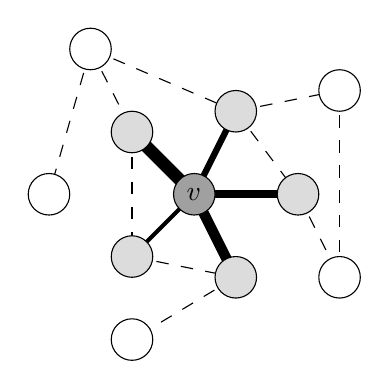
\begin{tikzpicture}[x=0.75pt,y=0.75pt,yscale=-1,xscale=1]
%uncomment if require: \path (0,180); %set diagram left start at 0, and has height of 180

%Straight Lines [id:da5686945126074561] 
\draw [line width=4.5]    (110,55) -- (140,85) ;
%Straight Lines [id:da9604209522132989] 
\draw [line width=2.25]    (140,85) -- (160,45) ;
%Straight Lines [id:da37557239319608837] 
\draw [line width=3]    (140,85) -- (190,85) ;
%Straight Lines [id:da6300189028004446] 
\draw [line width=3.75]    (140,85) -- (160,125) ;
%Straight Lines [id:da7961671100503147] 
\draw [line width=1.5]    (110,115) -- (140,85) ;
%Straight Lines [id:da3914617106414984] 
\draw  [dash pattern={on 4.5pt off 4.5pt}]  (110,55) -- (110,115) ;
%Straight Lines [id:da07988436759828788] 
\draw  [dash pattern={on 4.5pt off 4.5pt}]  (160,45) -- (190,85) ;
%Straight Lines [id:da7974028440726391] 
\draw  [dash pattern={on 4.5pt off 4.5pt}]  (190,85) -- (210,125) ;
%Straight Lines [id:da9163453027130692] 
\draw  [dash pattern={on 4.5pt off 4.5pt}]  (210,35) -- (210,125) ;
%Straight Lines [id:da8269233974334222] 
\draw  [dash pattern={on 4.5pt off 4.5pt}]  (160,45) -- (210,35) ;
%Straight Lines [id:da4638034672823643] 
\draw  [dash pattern={on 4.5pt off 4.5pt}]  (110,115) -- (160,125) ;
%Straight Lines [id:da8106142104727672] 
\draw  [dash pattern={on 4.5pt off 4.5pt}]  (160,125) -- (110,155) ;
%Straight Lines [id:da18520110140050194] 
\draw  [dash pattern={on 4.5pt off 4.5pt}]  (90,15) -- (70,85) ;
%Straight Lines [id:da625081015703862] 
\draw  [dash pattern={on 4.5pt off 4.5pt}]  (90,15) -- (160,45) ;
%Straight Lines [id:da82285820802776] 
\draw  [dash pattern={on 4.5pt off 4.5pt}]  (90,15) -- (111.24,56.72) ;
%Shape: Circle [id:dp9141923177042026] 
\draw  [fill={rgb, 255:red, 160; green, 160; blue, 160 }  ,fill opacity=1 ] (130,85) .. controls (130,79.48) and (134.48,75) .. (140,75) .. controls (145.52,75) and (150,79.48) .. (150,85) .. controls (150,90.52) and (145.52,95) .. (140,95) .. controls (134.48,95) and (130,90.52) .. (130,85) -- cycle ;
%Shape: Circle [id:dp18272847458947417] 
\draw  [fill={rgb, 255:red, 220; green, 220; blue, 220 }  ,fill opacity=1 ] (150,45) .. controls (150,39.48) and (154.48,35) .. (160,35) .. controls (165.52,35) and (170,39.48) .. (170,45) .. controls (170,50.52) and (165.52,55) .. (160,55) .. controls (154.48,55) and (150,50.52) .. (150,45) -- cycle ;
%Shape: Circle [id:dp6485883310805953] 
\draw  [fill={rgb, 255:red, 220; green, 220; blue, 220 }  ,fill opacity=1 ] (180,85) .. controls (180,79.48) and (184.48,75) .. (190,75) .. controls (195.52,75) and (200,79.48) .. (200,85) .. controls (200,90.52) and (195.52,95) .. (190,95) .. controls (184.48,95) and (180,90.52) .. (180,85) -- cycle ;
%Shape: Circle [id:dp4567157214251971] 
\draw  [fill={rgb, 255:red, 220; green, 220; blue, 220 }  ,fill opacity=1 ] (150,125) .. controls (150,119.48) and (154.48,115) .. (160,115) .. controls (165.52,115) and (170,119.48) .. (170,125) .. controls (170,130.52) and (165.52,135) .. (160,135) .. controls (154.48,135) and (150,130.52) .. (150,125) -- cycle ;
%Shape: Circle [id:dp9772039662669827] 
\draw  [fill={rgb, 255:red, 220; green, 220; blue, 220 }  ,fill opacity=1 ] (100,115) .. controls (100,109.48) and (104.48,105) .. (110,105) .. controls (115.52,105) and (120,109.48) .. (120,115) .. controls (120,120.52) and (115.52,125) .. (110,125) .. controls (104.48,125) and (100,120.52) .. (100,115) -- cycle ;
%Shape: Circle [id:dp849968227587317] 
\draw  [fill={rgb, 255:red, 220; green, 220; blue, 220 }  ,fill opacity=1 ] (100,55) .. controls (100,49.48) and (104.48,45) .. (110,45) .. controls (115.52,45) and (120,49.48) .. (120,55) .. controls (120,60.52) and (115.52,65) .. (110,65) .. controls (104.48,65) and (100,60.52) .. (100,55) -- cycle ;
%Shape: Circle [id:dp3852456165614402] 
\draw  [fill={rgb, 255:red, 255; green, 255; blue, 255 }  ,fill opacity=1 ] (60,85) .. controls (60,79.48) and (64.48,75) .. (70,75) .. controls (75.52,75) and (80,79.48) .. (80,85) .. controls (80,90.52) and (75.52,95) .. (70,95) .. controls (64.48,95) and (60,90.52) .. (60,85) -- cycle ;
%Shape: Circle [id:dp2002495564114657] 
\draw  [fill={rgb, 255:red, 255; green, 255; blue, 255 }  ,fill opacity=1 ] (80,15) .. controls (80,9.48) and (84.48,5) .. (90,5) .. controls (95.52,5) and (100,9.48) .. (100,15) .. controls (100,20.52) and (95.52,25) .. (90,25) .. controls (84.48,25) and (80,20.52) .. (80,15) -- cycle ;
%Shape: Circle [id:dp11701891156215805] 
\draw  [fill={rgb, 255:red, 255; green, 255; blue, 255 }  ,fill opacity=1 ] (200,35) .. controls (200,29.48) and (204.48,25) .. (210,25) .. controls (215.52,25) and (220,29.48) .. (220,35) .. controls (220,40.52) and (215.52,45) .. (210,45) .. controls (204.48,45) and (200,40.52) .. (200,35) -- cycle ;
%Shape: Circle [id:dp7052954164459615] 
\draw  [fill={rgb, 255:red, 255; green, 255; blue, 255 }  ,fill opacity=1 ] (200,125) .. controls (200,119.48) and (204.48,115) .. (210,115) .. controls (215.52,115) and (220,119.48) .. (220,125) .. controls (220,130.52) and (215.52,135) .. (210,135) .. controls (204.48,135) and (200,130.52) .. (200,125) -- cycle ;
%Shape: Circle [id:dp9425951388234] 
\draw  [fill={rgb, 255:red, 255; green, 255; blue, 255 }  ,fill opacity=1 ] (100,155) .. controls (100,149.48) and (104.48,145) .. (110,145) .. controls (115.52,145) and (120,149.48) .. (120,155) .. controls (120,160.52) and (115.52,165) .. (110,165) .. controls (104.48,165) and (100,160.52) .. (100,155) -- cycle ;

% Text Node
\draw (135,81) node [anchor=north west][inner sep=0.75pt]    {$v$};


\end{tikzpicture}}
    \caption{An example of node attention. Note that edge thickness is not related to the strength of the connection between node $v$ (in dark grey) and its neighbors (in light grey), but it represents the degree of similarity between the node states, quantified in a probabilistic sense by the attention score. Dashed edges connect nodes that are not involved in the attention score computation.}
    \label{fig:attention}
\end{figure*}

\paragraph{Node Sampling}
Node sampling is a technique used when learning on large graphs to ensure computational efficiency. When the number of nodes in a graph is large, and nodes are densely connected among themselves, computing neighborhood aggregation may become very expensive or even intractable. The most straightforward method to address this issue is to randomly sample a predefined number of nodes to aggregate, rather than using the whole neighborhood. This basic strategy can be refined by using more sophisticated techniques such as importance sampling \citep{gallicchio2020fastdeepgnn}, or even extended to sampling a bounded number of nodes which are not necessarily in the immediate neighborhood of the current node \citep{hamilton2017graphsage}. The latter requires to add fictitious edges between the current node and nodes at farther distances, in order to treat them as standard neighbors. This way, global information about the graph can be incorporated more directly, as compared to message passing.

\begin{figure*}[h!]
    \centering
    \resizebox{.35\textwidth}{!}{

\tikzset{every picture/.style={line width=0.75pt}} %set default line width to 0.75pt        

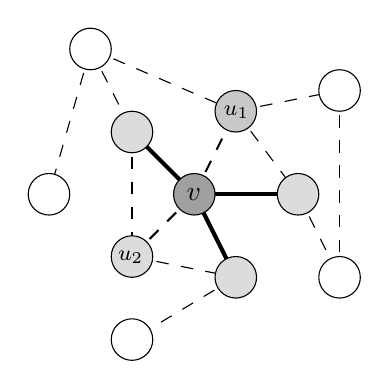
\begin{tikzpicture}[x=0.75pt,y=0.75pt,yscale=-1,xscale=1]
%uncomment if require: \path (0,180); %set diagram left start at 0, and has height of 180

%Straight Lines [id:da9928972582367306] 
\draw [line width=1.5]    (110,55) -- (140,85) ;
%Straight Lines [id:da7590045228035791] 
\draw [line width=0.75]  [dash pattern={on 4.5pt off 4.5pt}]  (140,85) -- (160,45) ;
%Straight Lines [id:da9311764026080076] 
\draw [line width=1.5]    (140,85) -- (190,85) ;
%Straight Lines [id:da7051144357210035] 
\draw [line width=1.5]    (140,85) -- (160,125) ;
%Straight Lines [id:da9499976233652532] 
\draw [line width=0.75]  [dash pattern={on 4.5pt off 4.5pt}]  (110,115) -- (140,85) ;
%Straight Lines [id:da6071610287175291] 
\draw  [dash pattern={on 4.5pt off 4.5pt}]  (110,55) -- (110,115) ;
%Straight Lines [id:da458862675888432] 
\draw  [dash pattern={on 4.5pt off 4.5pt}]  (160,45) -- (190,85) ;
%Straight Lines [id:da03442786949532706] 
\draw  [dash pattern={on 4.5pt off 4.5pt}]  (190,85) -- (210,125) ;
%Straight Lines [id:da1577597063925078] 
\draw  [dash pattern={on 4.5pt off 4.5pt}]  (210,35) -- (210,125) ;
%Straight Lines [id:da4513425022479223] 
\draw  [dash pattern={on 4.5pt off 4.5pt}]  (160,45) -- (210,35) ;
%Straight Lines [id:da9391313397847703] 
\draw  [dash pattern={on 4.5pt off 4.5pt}]  (110,115) -- (160,125) ;
%Straight Lines [id:da1766664603992849] 
\draw  [dash pattern={on 4.5pt off 4.5pt}]  (160,125) -- (110,155) ;
%Straight Lines [id:da38513478626684483] 
\draw  [dash pattern={on 4.5pt off 4.5pt}]  (90,15) -- (70,85) ;
%Straight Lines [id:da5306220988073596] 
\draw  [dash pattern={on 4.5pt off 4.5pt}]  (90,15) -- (160,45) ;
%Straight Lines [id:da6886418274825212] 
\draw  [dash pattern={on 4.5pt off 4.5pt}]  (90,15) -- (111.24,56.72) ;
%Shape: Circle [id:dp771344607660861] 
\draw  [fill={rgb, 255:red, 160; green, 160; blue, 160 }  ,fill opacity=1 ] (130,85) .. controls (130,79.48) and (134.48,75) .. (140,75) .. controls (145.52,75) and (150,79.48) .. (150,85) .. controls (150,90.52) and (145.52,95) .. (140,95) .. controls (134.48,95) and (130,90.52) .. (130,85) -- cycle ;
%Shape: Circle [id:dp27537395956973] 
\draw  [fill={rgb, 255:red, 200; green, 200; blue, 200 }  ,fill opacity=1 ] (150,45) .. controls (150,39.48) and (154.48,35) .. (160,35) .. controls (165.52,35) and (170,39.48) .. (170,45) .. controls (170,50.52) and (165.52,55) .. (160,55) .. controls (154.48,55) and (150,50.52) .. (150,45) -- cycle ;
%Shape: Circle [id:dp9311025651782232] 
\draw  [fill={rgb, 255:red, 220; green, 220; blue, 220 }  ,fill opacity=1 ] (180,85) .. controls (180,79.48) and (184.48,75) .. (190,75) .. controls (195.52,75) and (200,79.48) .. (200,85) .. controls (200,90.52) and (195.52,95) .. (190,95) .. controls (184.48,95) and (180,90.52) .. (180,85) -- cycle ;
%Shape: Circle [id:dp3681889727661305] 
\draw  [fill={rgb, 255:red, 220; green, 220; blue, 220 }  ,fill opacity=1 ] (150,125) .. controls (150,119.48) and (154.48,115) .. (160,115) .. controls (165.52,115) and (170,119.48) .. (170,125) .. controls (170,130.52) and (165.52,135) .. (160,135) .. controls (154.48,135) and (150,130.52) .. (150,125) -- cycle ;
%Shape: Circle [id:dp4411140386684782] 
\draw  [fill={rgb, 255:red, 220; green, 220; blue, 220 }  ,fill opacity=1 ] (100,115) .. controls (100,109.48) and (104.48,105) .. (110,105) .. controls (115.52,105) and (120,109.48) .. (120,115) .. controls (120,120.52) and (115.52,125) .. (110,125) .. controls (104.48,125) and (100,120.52) .. (100,115) -- cycle ;
%Shape: Circle [id:dp22700882921378018] 
\draw  [fill={rgb, 255:red, 220; green, 220; blue, 220 }  ,fill opacity=1 ] (100,55) .. controls (100,49.48) and (104.48,45) .. (110,45) .. controls (115.52,45) and (120,49.48) .. (120,55) .. controls (120,60.52) and (115.52,65) .. (110,65) .. controls (104.48,65) and (100,60.52) .. (100,55) -- cycle ;
%Shape: Circle [id:dp1737413883891752] 
\draw  [fill={rgb, 255:red, 255; green, 255; blue, 255 }  ,fill opacity=1 ] (60,85) .. controls (60,79.48) and (64.48,75) .. (70,75) .. controls (75.52,75) and (80,79.48) .. (80,85) .. controls (80,90.52) and (75.52,95) .. (70,95) .. controls (64.48,95) and (60,90.52) .. (60,85) -- cycle ;
%Shape: Circle [id:dp9017509150985334] 
\draw  [fill={rgb, 255:red, 255; green, 255; blue, 255 }  ,fill opacity=1 ] (80,15) .. controls (80,9.48) and (84.48,5) .. (90,5) .. controls (95.52,5) and (100,9.48) .. (100,15) .. controls (100,20.52) and (95.52,25) .. (90,25) .. controls (84.48,25) and (80,20.52) .. (80,15) -- cycle ;
%Shape: Circle [id:dp1681742526969252] 
\draw  [fill={rgb, 255:red, 255; green, 255; blue, 255 }  ,fill opacity=1 ] (200,35) .. controls (200,29.48) and (204.48,25) .. (210,25) .. controls (215.52,25) and (220,29.48) .. (220,35) .. controls (220,40.52) and (215.52,45) .. (210,45) .. controls (204.48,45) and (200,40.52) .. (200,35) -- cycle ;
%Shape: Circle [id:dp32379455826600156] 
\draw  [fill={rgb, 255:red, 255; green, 255; blue, 255 }  ,fill opacity=1 ] (200,125) .. controls (200,119.48) and (204.48,115) .. (210,115) .. controls (215.52,115) and (220,119.48) .. (220,125) .. controls (220,130.52) and (215.52,135) .. (210,135) .. controls (204.48,135) and (200,130.52) .. (200,125) -- cycle ;
%Shape: Circle [id:dp8687072580412498] 
\draw  [fill={rgb, 255:red, 255; green, 255; blue, 255 }  ,fill opacity=1 ] (100,155) .. controls (100,149.48) and (104.48,145) .. (110,145) .. controls (115.52,145) and (120,149.48) .. (120,155) .. controls (120,160.52) and (115.52,165) .. (110,165) .. controls (104.48,165) and (100,160.52) .. (100,155) -- cycle ;

% Text Node
\draw (135,81) node [anchor=north west][inner sep=0.75pt]    {$v$};
% Text Node
\draw (153,41) node [anchor=north west][inner sep=0.75pt]  [font=\footnotesize]  {$u_{1}$};
% Text Node
\draw (102,111) node [anchor=north west][inner sep=0.75pt]  [font=\footnotesize]  {$u_{2}$};


\end{tikzpicture}}
    \caption{An example of node sampling. We focus on a node $v$ (in dark grey), and its neighbors (in light grey). Dashed edges connect nodes that are not involved in the neighborhood aggregation; notice how nodes $u_1$ and $u_2$ are excluded from the neighborhood aggregation, even though they are effectively neighbors of $v$.}
    \label{fig:sampling}
\end{figure*}

\subsection{Readout Layers}
As we have seen, the application of $L$ \gls{dgn} layers to a graph $\GraphU{G}$ yields $L$ hidden states per node, each one composed with a progressively broad context. In node classification or regression tasks, these are combined by a \emph{hidden state readout} function to obtain a unique hidden state to use as input of the output function, which emits a prediction for every node. Specifically, a hidden state readout function $\Fun{R'}$ computes a \keyword{node representation} (or \keyword{node embeddings}) $\StateVector{v}{*}$ for each node as follows:
$$\StateVector{v}{*} = \Op{R}_{v}\Par{\Set{\StateVector{v}{\ell} \mid \ell = 1, \ldots, L}},\;  \forall v \in \Nodes{g}. $$
Notice that, when aggregating hidden states, one can exploit the fact that the number of layers is fixed beforehand in feed-forward \gls{dgn} architectures, and that the hidden states are ordered depth-wise. Thus, the aggregation need not to be permutation-invariant. Usual choices of $\Op{R}_{v}$ include concatenation, weighted average (where the mixing weights can also be learned), \gls{rnn}s, or just selecting the hidden state at the last layer. The node representations are then fed to an output layer or downstream network, which computes node-wise outputs:
$$\Elem{o}{v} = g(\StateVector{v}{*}),\; \forall v \in \Nodes{g},$$
where $\Elem{o}{v} \in \Real^y$ and $g$ can be any arbitrarily complex neural network as usual. A visual example of the process for a single node is shown in Figure \ref{fig:node-readout}.
\begin{figure*}[h!]
    \centering
    \resizebox{.6\textwidth}{!}{

\tikzset{every picture/.style={line width=0.75pt}} %set default line width to 0.75pt        

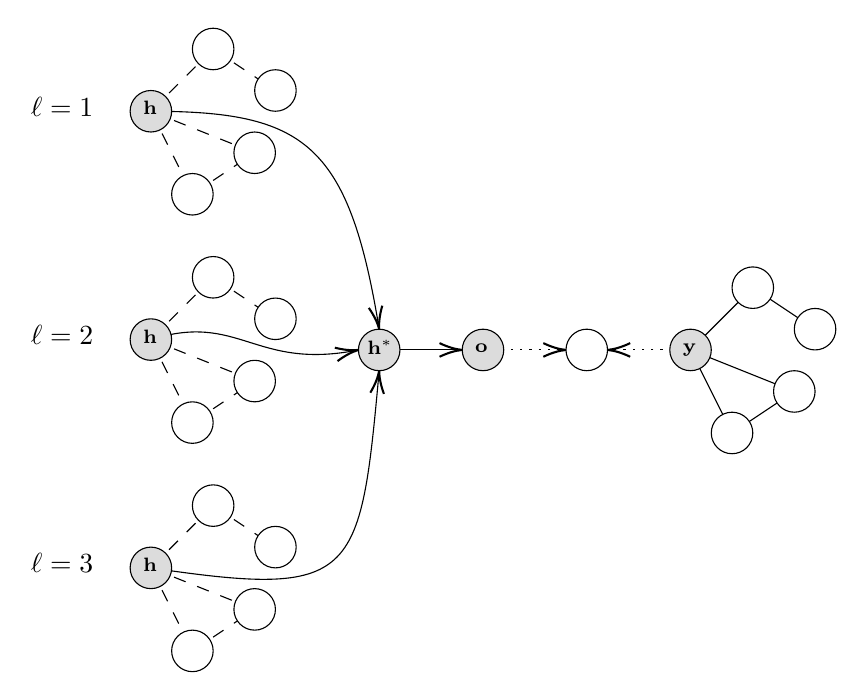
\begin{tikzpicture}[x=0.75pt,y=0.75pt,yscale=-1,xscale=1]
%uncomment if require: \path (0,325); %set diagram left start at 0, and has height of 325

%Straight Lines [id:da8021808052596502] 
\draw    (180,165) -- (218,165) ;
\draw [shift={(220,165)}, rotate = 180] [color={rgb, 255:red, 0; green, 0; blue, 0 }  ][line width=0.75]    (10.93,-3.29) .. controls (6.95,-1.4) and (3.31,-0.3) .. (0,0) .. controls (3.31,0.3) and (6.95,1.4) .. (10.93,3.29)   ;
%Straight Lines [id:da8262157575030338] 
\draw  [dash pattern={on 4.5pt off 4.5pt}]  (100,130) -- (70,160) ;
%Straight Lines [id:da09418463263497934] 
\draw  [dash pattern={on 4.5pt off 4.5pt}]  (70,160) -- (90,200) ;
%Straight Lines [id:da04169663842617122] 
\draw  [dash pattern={on 4.5pt off 4.5pt}]  (70,160) -- (120,180) ;
%Straight Lines [id:da9649034616072283] 
\draw  [dash pattern={on 4.5pt off 4.5pt}]  (90,200) -- (120,180) ;
%Straight Lines [id:da9180072651610127] 
\draw  [dash pattern={on 4.5pt off 4.5pt}]  (100,130) -- (130,150) ;
%Shape: Circle [id:dp5528328090096748] 
\draw  [fill={rgb, 255:red, 255; green, 255; blue, 255 }  ,fill opacity=1 ] (80,200) .. controls (80,194.48) and (84.48,190) .. (90,190) .. controls (95.52,190) and (100,194.48) .. (100,200) .. controls (100,205.52) and (95.52,210) .. (90,210) .. controls (84.48,210) and (80,205.52) .. (80,200) -- cycle ;
%Shape: Circle [id:dp9881598411642218] 
\draw  [fill={rgb, 255:red, 255; green, 255; blue, 255 }  ,fill opacity=1 ] (110,180) .. controls (110,174.48) and (114.48,170) .. (120,170) .. controls (125.52,170) and (130,174.48) .. (130,180) .. controls (130,185.52) and (125.52,190) .. (120,190) .. controls (114.48,190) and (110,185.52) .. (110,180) -- cycle ;
%Shape: Circle [id:dp8848288279392054] 
\draw  [fill={rgb, 255:red, 255; green, 255; blue, 255 }  ,fill opacity=1 ] (120,150) .. controls (120,144.48) and (124.48,140) .. (130,140) .. controls (135.52,140) and (140,144.48) .. (140,150) .. controls (140,155.52) and (135.52,160) .. (130,160) .. controls (124.48,160) and (120,155.52) .. (120,150) -- cycle ;
%Shape: Circle [id:dp4318188413506394] 
\draw  [fill={rgb, 255:red, 255; green, 255; blue, 255 }  ,fill opacity=1 ] (90,130) .. controls (90,124.48) and (94.48,120) .. (100,120) .. controls (105.52,120) and (110,124.48) .. (110,130) .. controls (110,135.52) and (105.52,140) .. (100,140) .. controls (94.48,140) and (90,135.52) .. (90,130) -- cycle ;
%Straight Lines [id:da45587472919699423] 
\draw  [dash pattern={on 4.5pt off 4.5pt}]  (100,20) -- (70,50) ;
%Straight Lines [id:da3322812526365526] 
\draw  [dash pattern={on 4.5pt off 4.5pt}]  (70,50) -- (90,90) ;
%Straight Lines [id:da060418746819522307] 
\draw  [dash pattern={on 4.5pt off 4.5pt}]  (70,50) -- (120,70) ;
%Straight Lines [id:da6519027932168682] 
\draw  [dash pattern={on 4.5pt off 4.5pt}]  (90,90) -- (120,70) ;
%Straight Lines [id:da10647901279823291] 
\draw  [dash pattern={on 4.5pt off 4.5pt}]  (100,20) -- (130,40) ;
%Shape: Circle [id:dp6069852564048885] 
\draw  [fill={rgb, 255:red, 255; green, 255; blue, 255 }  ,fill opacity=1 ] (80,90) .. controls (80,84.48) and (84.48,80) .. (90,80) .. controls (95.52,80) and (100,84.48) .. (100,90) .. controls (100,95.52) and (95.52,100) .. (90,100) .. controls (84.48,100) and (80,95.52) .. (80,90) -- cycle ;
%Shape: Circle [id:dp28187241585395206] 
\draw  [fill={rgb, 255:red, 255; green, 255; blue, 255 }  ,fill opacity=1 ] (110,70) .. controls (110,64.48) and (114.48,60) .. (120,60) .. controls (125.52,60) and (130,64.48) .. (130,70) .. controls (130,75.52) and (125.52,80) .. (120,80) .. controls (114.48,80) and (110,75.52) .. (110,70) -- cycle ;
%Shape: Circle [id:dp36091441623126763] 
\draw  [fill={rgb, 255:red, 255; green, 255; blue, 255 }  ,fill opacity=1 ] (120,40) .. controls (120,34.48) and (124.48,30) .. (130,30) .. controls (135.52,30) and (140,34.48) .. (140,40) .. controls (140,45.52) and (135.52,50) .. (130,50) .. controls (124.48,50) and (120,45.52) .. (120,40) -- cycle ;
%Shape: Circle [id:dp48327367752052597] 
\draw  [fill={rgb, 255:red, 255; green, 255; blue, 255 }  ,fill opacity=1 ] (90,20) .. controls (90,14.48) and (94.48,10) .. (100,10) .. controls (105.52,10) and (110,14.48) .. (110,20) .. controls (110,25.52) and (105.52,30) .. (100,30) .. controls (94.48,30) and (90,25.52) .. (90,20) -- cycle ;
%Straight Lines [id:da6727907472991814] 
\draw  [dash pattern={on 4.5pt off 4.5pt}]  (100,240) -- (70,270) ;
%Straight Lines [id:da4536448975686458] 
\draw  [dash pattern={on 4.5pt off 4.5pt}]  (70,270) -- (90,310) ;
%Straight Lines [id:da46318384192507667] 
\draw  [dash pattern={on 4.5pt off 4.5pt}]  (70,270) -- (120,290) ;
%Straight Lines [id:da26138928549207874] 
\draw  [dash pattern={on 4.5pt off 4.5pt}]  (90,310) -- (120,290) ;
%Straight Lines [id:da25645750289270874] 
\draw  [dash pattern={on 4.5pt off 4.5pt}]  (100,240) -- (130,260) ;
%Shape: Circle [id:dp29709464392681206] 
\draw  [fill={rgb, 255:red, 255; green, 255; blue, 255 }  ,fill opacity=1 ] (80,310) .. controls (80,304.48) and (84.48,300) .. (90,300) .. controls (95.52,300) and (100,304.48) .. (100,310) .. controls (100,315.52) and (95.52,320) .. (90,320) .. controls (84.48,320) and (80,315.52) .. (80,310) -- cycle ;
%Shape: Circle [id:dp5007793010043322] 
\draw  [fill={rgb, 255:red, 255; green, 255; blue, 255 }  ,fill opacity=1 ] (110,290) .. controls (110,284.48) and (114.48,280) .. (120,280) .. controls (125.52,280) and (130,284.48) .. (130,290) .. controls (130,295.52) and (125.52,300) .. (120,300) .. controls (114.48,300) and (110,295.52) .. (110,290) -- cycle ;
%Shape: Circle [id:dp7842479967392513] 
\draw  [fill={rgb, 255:red, 255; green, 255; blue, 255 }  ,fill opacity=1 ] (120,260) .. controls (120,254.48) and (124.48,250) .. (130,250) .. controls (135.52,250) and (140,254.48) .. (140,260) .. controls (140,265.52) and (135.52,270) .. (130,270) .. controls (124.48,270) and (120,265.52) .. (120,260) -- cycle ;
%Shape: Circle [id:dp08352653569945168] 
\draw  [fill={rgb, 255:red, 255; green, 255; blue, 255 }  ,fill opacity=1 ] (90,240) .. controls (90,234.48) and (94.48,230) .. (100,230) .. controls (105.52,230) and (110,234.48) .. (110,240) .. controls (110,245.52) and (105.52,250) .. (100,250) .. controls (94.48,250) and (90,245.52) .. (90,240) -- cycle ;
%Straight Lines [id:da08172279961172113] 
\draw    (360,135) -- (330,165) ;
%Straight Lines [id:da5964854301837534] 
\draw    (330,165) -- (350,205) ;
%Straight Lines [id:da705675390083226] 
\draw    (330,165) -- (380,185) ;
%Straight Lines [id:da657700600239705] 
\draw    (350,205) -- (380,185) ;
%Straight Lines [id:da3851868502745348] 
\draw    (360,135) -- (390,155) ;
%Shape: Circle [id:dp724750055071185] 
\draw  [fill={rgb, 255:red, 255; green, 255; blue, 255 }  ,fill opacity=1 ] (340,205) .. controls (340,199.48) and (344.48,195) .. (350,195) .. controls (355.52,195) and (360,199.48) .. (360,205) .. controls (360,210.52) and (355.52,215) .. (350,215) .. controls (344.48,215) and (340,210.52) .. (340,205) -- cycle ;
%Shape: Circle [id:dp45589554777220975] 
\draw  [fill={rgb, 255:red, 255; green, 255; blue, 255 }  ,fill opacity=1 ] (370,185) .. controls (370,179.48) and (374.48,175) .. (380,175) .. controls (385.52,175) and (390,179.48) .. (390,185) .. controls (390,190.52) and (385.52,195) .. (380,195) .. controls (374.48,195) and (370,190.52) .. (370,185) -- cycle ;
%Shape: Circle [id:dp8985548220725617] 
\draw  [fill={rgb, 255:red, 255; green, 255; blue, 255 }  ,fill opacity=1 ] (380,155) .. controls (380,149.48) and (384.48,145) .. (390,145) .. controls (395.52,145) and (400,149.48) .. (400,155) .. controls (400,160.52) and (395.52,165) .. (390,165) .. controls (384.48,165) and (380,160.52) .. (380,155) -- cycle ;
%Shape: Circle [id:dp5150110802600167] 
\draw  [fill={rgb, 255:red, 255; green, 255; blue, 255 }  ,fill opacity=1 ] (350,135) .. controls (350,129.48) and (354.48,125) .. (360,125) .. controls (365.52,125) and (370,129.48) .. (370,135) .. controls (370,140.52) and (365.52,145) .. (360,145) .. controls (354.48,145) and (350,140.52) .. (350,135) -- cycle ;
%Curve Lines [id:da6191074648732291] 
\draw    (70,50) .. controls (143.43,50.05) and (165.08,64.9) .. (179.78,153.66) ;
\draw [shift={(180,155)}, rotate = 260.72] [color={rgb, 255:red, 0; green, 0; blue, 0 }  ][line width=0.75]    (10.93,-3.29) .. controls (6.95,-1.4) and (3.31,-0.3) .. (0,0) .. controls (3.31,0.3) and (6.95,1.4) .. (10.93,3.29)   ;
%Curve Lines [id:da12167346141027413] 
\draw    (70,160) .. controls (112.37,146.68) and (119.66,174.48) .. (168.51,165.29) ;
\draw [shift={(170,165)}, rotate = 528.6800000000001] [color={rgb, 255:red, 0; green, 0; blue, 0 }  ][line width=0.75]    (10.93,-3.29) .. controls (6.95,-1.4) and (3.31,-0.3) .. (0,0) .. controls (3.31,0.3) and (6.95,1.4) .. (10.93,3.29)   ;
%Curve Lines [id:da6495417615361903] 
\draw    (70,270) .. controls (168.8,284.68) and (170.78,275.34) .. (179.86,176.5) ;
\draw [shift={(180,175)}, rotate = 455.24] [color={rgb, 255:red, 0; green, 0; blue, 0 }  ][line width=0.75]    (10.93,-3.29) .. controls (6.95,-1.4) and (3.31,-0.3) .. (0,0) .. controls (3.31,0.3) and (6.95,1.4) .. (10.93,3.29)   ;
%Shape: Circle [id:dp8473323519447842] 
\draw  [fill={rgb, 255:red, 220; green, 220; blue, 220 }  ,fill opacity=1 ] (60,160) .. controls (60,154.48) and (64.48,150) .. (70,150) .. controls (75.52,150) and (80,154.48) .. (80,160) .. controls (80,165.52) and (75.52,170) .. (70,170) .. controls (64.48,170) and (60,165.52) .. (60,160) -- cycle ;
%Shape: Circle [id:dp877285523901683] 
\draw  [fill={rgb, 255:red, 220; green, 220; blue, 220 }  ,fill opacity=1 ] (60,50) .. controls (60,44.48) and (64.48,40) .. (70,40) .. controls (75.52,40) and (80,44.48) .. (80,50) .. controls (80,55.52) and (75.52,60) .. (70,60) .. controls (64.48,60) and (60,55.52) .. (60,50) -- cycle ;
%Shape: Circle [id:dp5471945476486635] 
\draw  [fill={rgb, 255:red, 220; green, 220; blue, 220 }  ,fill opacity=1 ] (60,270) .. controls (60,264.48) and (64.48,260) .. (70,260) .. controls (75.52,260) and (80,264.48) .. (80,270) .. controls (80,275.52) and (75.52,280) .. (70,280) .. controls (64.48,280) and (60,275.52) .. (60,270) -- cycle ;
%Straight Lines [id:da5747740801523578] 
\draw  [dash pattern={on 0.84pt off 2.51pt}]  (230,165) -- (268,165) ;
\draw [shift={(270,165)}, rotate = 180] [color={rgb, 255:red, 0; green, 0; blue, 0 }  ][line width=0.75]    (10.93,-3.29) .. controls (6.95,-1.4) and (3.31,-0.3) .. (0,0) .. controls (3.31,0.3) and (6.95,1.4) .. (10.93,3.29)   ;
%Straight Lines [id:da7736106844919413] 
\draw  [dash pattern={on 0.84pt off 2.51pt}]  (330,165) -- (292,165) ;
\draw [shift={(290,165)}, rotate = 360] [color={rgb, 255:red, 0; green, 0; blue, 0 }  ][line width=0.75]    (10.93,-3.29) .. controls (6.95,-1.4) and (3.31,-0.3) .. (0,0) .. controls (3.31,0.3) and (6.95,1.4) .. (10.93,3.29)   ;
%Shape: Circle [id:dp8719481497855568] 
\draw  [fill={rgb, 255:red, 220; green, 220; blue, 220 }  ,fill opacity=1 ] (170,165) .. controls (170,159.48) and (174.48,155) .. (180,155) .. controls (185.52,155) and (190,159.48) .. (190,165) .. controls (190,170.52) and (185.52,175) .. (180,175) .. controls (174.48,175) and (170,170.52) .. (170,165) -- cycle ;
%Shape: Circle [id:dp3225900460836928] 
\draw  [fill={rgb, 255:red, 255; green, 255; blue, 255 }  ,fill opacity=1 ] (270,165) .. controls (270,159.48) and (274.48,155) .. (280,155) .. controls (285.52,155) and (290,159.48) .. (290,165) .. controls (290,170.52) and (285.52,175) .. (280,175) .. controls (274.48,175) and (270,170.52) .. (270,165) -- cycle ;
%Shape: Circle [id:dp7781672542643503] 
\draw  [fill={rgb, 255:red, 220; green, 220; blue, 220 }  ,fill opacity=1 ] (320,165) .. controls (320,159.48) and (324.48,155) .. (330,155) .. controls (335.52,155) and (340,159.48) .. (340,165) .. controls (340,170.52) and (335.52,175) .. (330,175) .. controls (324.48,175) and (320,170.52) .. (320,165) -- cycle ;
%Shape: Circle [id:dp1531568176441671] 
\draw  [fill={rgb, 255:red, 220; green, 220; blue, 220 }  ,fill opacity=1 ] (220,165) .. controls (220,159.48) and (224.48,155) .. (230,155) .. controls (235.52,155) and (240,159.48) .. (240,165) .. controls (240,170.52) and (235.52,175) .. (230,175) .. controls (224.48,175) and (220,170.52) .. (220,165) -- cycle ;


% Text Node
\draw (273,160) node [anchor=north west][inner sep=0.75pt]  [font=\scriptsize]  {$\Loss$};
% Text Node
\draw (10.9,151.8) node [anchor=north west][inner sep=0.75pt]    {$\ell =2$};
% Text Node
\draw (10.9,261.8) node [anchor=north west][inner sep=0.75pt]    {$\ell =3$};
% Text Node
\draw (10.9,41.8) node [anchor=north west][inner sep=0.75pt]    {$\ell =1$};
% Text Node
\draw (65,44) node [anchor=north west][inner sep=0.75pt]  [font=\scriptsize]  {$\mathbf{h}$};
% Text Node
\draw (65,154) node [anchor=north west][inner sep=0.75pt]  [font=\scriptsize]  {$\mathbf{h}$};
% Text Node
\draw (65,264) node [anchor=north west][inner sep=0.75pt]  [font=\scriptsize]  {$\mathbf{h}$};
% Text Node
\draw (173,159) node [anchor=north west][inner sep=0.75pt]  [font=\scriptsize]  {$\mathbf{h}^{*}$};
% Text Node
\draw (325,161) node [anchor=north west][inner sep=0.75pt]  [font=\scriptsize]  {$\mathbf{y}$};
% Text Node
\draw (225,161) node [anchor=north west][inner sep=0.75pt]  [font=\scriptsize]  {$\mathbf{o}$};


\end{tikzpicture}}
    \caption{The role of hidden state readout function in a node classification/regression task. Here, we focus on a single node $\StateVector{v}{\ell}$, where we drop the subscripts to avoid visual cluttering. Grey nodes replace the $[v]$ subscript. The hidden state readout function creates a node representation $\StateVector{v}{*}$ by combining its three hidden states (one for each layer). Successively, the node representation is turned into an output by an output layer, and compared by the loss function to the same node $\Elem{y}{v}$ in the isomorphic target graph. This operation is repeated for every node in the graph.}
    \label{fig:node-readout}
\end{figure*}
In graph classification or regression tasks, the node representations computed by a node readout function are aggregated once more by a \emph{graph readout} function, to compute a \keyword{graph representation} (or \keyword{graph embedding}) $\GraphRepr{g}$, \ie a vector representing the entire graph. Differently from the hidden state readout, the readout function must necessarily be permutation-invariant, since there are no guarantees about the number of graph nodes. Specifically, a graph readout function $\Fun{R}$ computes the embedding of graph $\GraphU{g}$ as follows:
$$\GraphRepr{g} = \GraphReadout{g}\Par{\Set{\StateVector{v}{*} \mid v \in \Nodes{g}}}.$$
Typical readouts for \glspl{dgn} include simple functions such sum, mean, max, or more complex aggregators such as deep sets models \citep{zaheer2017deepsets}. Finally, the graph embedding is fed to an output layer or a downstream network to compute the associated output:
$$\Vector{o} = g(\GraphRepr{g}).$$
\begin{figure*}[h!]
    \centering
    \resizebox{.6\textwidth}{!}{

\tikzset{every picture/.style={line width=0.75pt}} %set default line width to 0.75pt

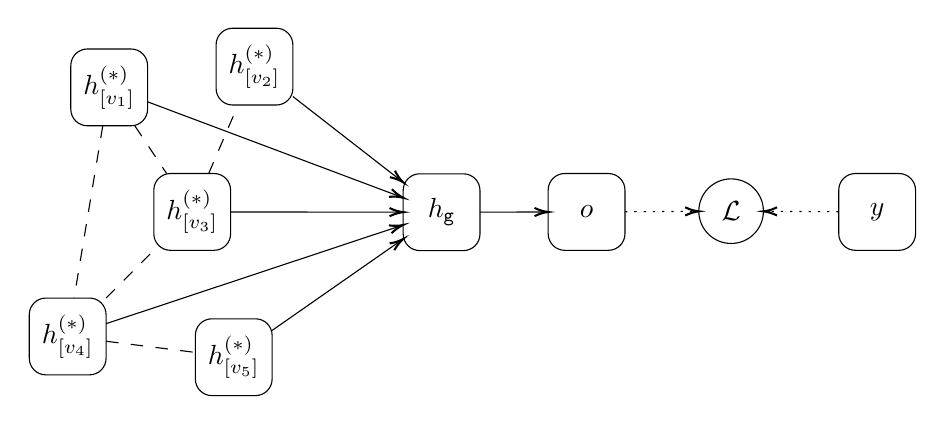
\begin{tikzpicture}[x=0.75pt,y=0.75pt,yscale=-1,xscale=1]
%uncomment if require: \path (0,300); %set diagram left start at 0, and has height of 300


% Text Node
\draw    (37.86,185.86) .. controls (37.86,181.44) and (41.44,177.86) .. (45.86,177.86) -- (66.86,177.86) .. controls (71.28,177.86) and (74.86,181.44) .. (74.86,185.86) -- (74.86,206.86) .. controls (74.86,211.28) and (71.28,214.86) .. (66.86,214.86) -- (45.86,214.86) .. controls (41.44,214.86) and (37.86,211.28) .. (37.86,206.86) -- cycle  ;
\draw (56.36,196.36) node   [align=left] {\begin{minipage}[lt]{22.249600830078126pt}\setlength\topsep{0pt}
\begin{center}
$\displaystyle \boldsymbol{h}^{( *)}_{[ v_{4}]}$
\end{center}

\end{minipage}};
% Text Node
\draw    (57.86,65.86) .. controls (57.86,61.44) and (61.44,57.86) .. (65.86,57.86) -- (86.86,57.86) .. controls (91.28,57.86) and (94.86,61.44) .. (94.86,65.86) -- (94.86,86.86) .. controls (94.86,91.28) and (91.28,94.86) .. (86.86,94.86) -- (65.86,94.86) .. controls (61.44,94.86) and (57.86,91.28) .. (57.86,86.86) -- cycle  ;
\draw (76.36,76.36) node   [align=left] {\begin{minipage}[lt]{22.249600830078126pt}\setlength\topsep{0pt}
\begin{center}
$\displaystyle \boldsymbol{h}^{( *)}_{[ v_{1}]}$
\end{center}

\end{minipage}};
% Text Node
\draw    (97.86,125.86) .. controls (97.86,121.44) and (101.44,117.86) .. (105.86,117.86) -- (126.86,117.86) .. controls (131.28,117.86) and (134.86,121.44) .. (134.86,125.86) -- (134.86,146.86) .. controls (134.86,151.28) and (131.28,154.86) .. (126.86,154.86) -- (105.86,154.86) .. controls (101.44,154.86) and (97.86,151.28) .. (97.86,146.86) -- cycle  ;
\draw (116.36,136.36) node   [align=left] {\begin{minipage}[lt]{22.249600830078126pt}\setlength\topsep{0pt}
\begin{center}
$\displaystyle \boldsymbol{h}^{( *)}_{[ v_{3}]}$
\end{center}

\end{minipage}};
% Text Node
\draw    (117.86,195.86) .. controls (117.86,191.44) and (121.44,187.86) .. (125.86,187.86) -- (146.86,187.86) .. controls (151.28,187.86) and (154.86,191.44) .. (154.86,195.86) -- (154.86,216.86) .. controls (154.86,221.28) and (151.28,224.86) .. (146.86,224.86) -- (125.86,224.86) .. controls (121.44,224.86) and (117.86,221.28) .. (117.86,216.86) -- cycle  ;
\draw (136.36,206.36) node   [align=left] {\begin{minipage}[lt]{22.249600830078126pt}\setlength\topsep{0pt}
\begin{center}
$\displaystyle \boldsymbol{h}^{( *)}_{[ v_{5}]}$
\end{center}

\end{minipage}};
% Text Node
\draw    (127.86,55.86) .. controls (127.86,51.44) and (131.44,47.86) .. (135.86,47.86) -- (156.86,47.86) .. controls (161.28,47.86) and (164.86,51.44) .. (164.86,55.86) -- (164.86,76.86) .. controls (164.86,81.28) and (161.28,84.86) .. (156.86,84.86) -- (135.86,84.86) .. controls (131.44,84.86) and (127.86,81.28) .. (127.86,76.86) -- cycle  ;
\draw (146.36,66.36) node   [align=left] {\begin{minipage}[lt]{22.249600830078126pt}\setlength\topsep{0pt}
\begin{center}
$\displaystyle \boldsymbol{h}^{( *)}_{[ v_{2}]}$
\end{center}

\end{minipage}};
% Text Node
\draw    (218,126) .. controls (218,121.58) and (221.58,118) .. (226,118) -- (247,118) .. controls (251.42,118) and (255,121.58) .. (255,126) -- (255,147) .. controls (255,151.42) and (251.42,155) .. (247,155) -- (226,155) .. controls (221.58,155) and (218,151.42) .. (218,147) -- cycle  ;
\draw (236.5,136.5) node   [align=left] {\begin{minipage}[lt]{22.249600830078126pt}\setlength\topsep{0pt}
\begin{center}
$\displaystyle \boldsymbol{h}_{\mathtt{g}}$
\end{center}

\end{minipage}};
% Text Node
\draw    (287.86,125.86) .. controls (287.86,121.44) and (291.44,117.86) .. (295.86,117.86) -- (316.86,117.86) .. controls (321.28,117.86) and (324.86,121.44) .. (324.86,125.86) -- (324.86,146.86) .. controls (324.86,151.28) and (321.28,154.86) .. (316.86,154.86) -- (295.86,154.86) .. controls (291.44,154.86) and (287.86,151.28) .. (287.86,146.86) -- cycle  ;
\draw (306.36,136.36) node   [align=left] {\begin{minipage}[lt]{22.249600830078126pt}\setlength\topsep{0pt}
\begin{center}
$\displaystyle \boldsymbol{o}$
\end{center}

\end{minipage}};
% Text Node
\draw    (376, 136) circle [x radius= 15.56, y radius= 15.56]   ;
\draw (376,136) node   [align=left] {\begin{minipage}[lt]{13.600000000000001pt}\setlength\topsep{0pt}
\begin{center}
$\displaystyle \mathcal{L}$
\end{center}

\end{minipage}};
% Text Node
\draw    (427.86,125.86) .. controls (427.86,121.44) and (431.44,117.86) .. (435.86,117.86) -- (456.86,117.86) .. controls (461.28,117.86) and (464.86,121.44) .. (464.86,125.86) -- (464.86,146.86) .. controls (464.86,151.28) and (461.28,154.86) .. (456.86,154.86) -- (435.86,154.86) .. controls (431.44,154.86) and (427.86,151.28) .. (427.86,146.86) -- cycle  ;
\draw (446.36,136.36) node   [align=left] {\begin{minipage}[lt]{22.249600830078126pt}\setlength\topsep{0pt}
\begin{center}
$\displaystyle \boldsymbol{y}$
\end{center}

\end{minipage}};
% Connection
\draw  [dash pattern={on 4.5pt off 4.5pt}]  (73.28,94.86) -- (59.44,177.86) ;
% Connection
\draw  [dash pattern={on 4.5pt off 4.5pt}]  (88.69,94.86) -- (104.03,117.86) ;
% Connection
\draw  [dash pattern={on 4.5pt off 4.5pt}]  (124.29,117.86) -- (138.43,84.86) ;
% Connection
\draw  [dash pattern={on 4.5pt off 4.5pt}]  (74.86,177.86) -- (97.86,154.86) ;
% Connection
\draw  [dash pattern={on 4.5pt off 4.5pt}]  (74.86,198.67) -- (117.86,204.05) ;
% Connection
\draw    (164.86,80.76) -- (216.42,120.88) ;
\draw [shift={(218,122.1)}, rotate = 217.89] [color={rgb, 255:red, 0; green, 0; blue, 0 }  ][line width=0.75]    (6.56,-1.97) .. controls (4.17,-0.84) and (1.99,-0.18) .. (0,0) .. controls (1.99,0.18) and (4.17,0.84) .. (6.56,1.97)   ;
% Connection
\draw    (134.86,136.38) -- (216,136.48) ;
\draw [shift={(218,136.48)}, rotate = 180.07] [color={rgb, 255:red, 0; green, 0; blue, 0 }  ][line width=0.75]    (6.56,-1.97) .. controls (4.17,-0.84) and (1.99,-0.18) .. (0,0) .. controls (1.99,0.18) and (4.17,0.84) .. (6.56,1.97)   ;
% Connection
\draw    (154.86,193.45) -- (216.36,150.55) ;
\draw [shift={(218,149.41)}, rotate = 505.1] [color={rgb, 255:red, 0; green, 0; blue, 0 }  ][line width=0.75]    (6.56,-1.97) .. controls (4.17,-0.84) and (1.99,-0.18) .. (0,0) .. controls (1.99,0.18) and (4.17,0.84) .. (6.56,1.97)   ;
% Connection
\draw    (74.86,190.21) -- (216.1,143.28) ;
\draw [shift={(218,142.65)}, rotate = 521.62] [color={rgb, 255:red, 0; green, 0; blue, 0 }  ][line width=0.75]    (6.56,-1.97) .. controls (4.17,-0.84) and (1.99,-0.18) .. (0,0) .. controls (1.99,0.18) and (4.17,0.84) .. (6.56,1.97)   ;
% Connection
\draw    (94.86,83.31) -- (216.13,128.85) ;
\draw [shift={(218,129.55)}, rotate = 200.57999999999998] [color={rgb, 255:red, 0; green, 0; blue, 0 }  ][line width=0.75]    (6.56,-1.97) .. controls (4.17,-0.84) and (1.99,-0.18) .. (0,0) .. controls (1.99,0.18) and (4.17,0.84) .. (6.56,1.97)   ;
% Connection
\draw    (255,136.46) -- (285.86,136.4) ;
\draw [shift={(287.86,136.4)}, rotate = 539.89] [color={rgb, 255:red, 0; green, 0; blue, 0 }  ][line width=0.75]    (6.56,-1.97) .. controls (4.17,-0.84) and (1.99,-0.18) .. (0,0) .. controls (1.99,0.18) and (4.17,0.84) .. (6.56,1.97)   ;
% Connection
\draw  [dash pattern={on 0.84pt off 2.51pt}]  (324.86,136.26) -- (358.44,136.09) ;
\draw [shift={(360.44,136.08)}, rotate = 539.7] [color={rgb, 255:red, 0; green, 0; blue, 0 }  ][line width=0.75]    (6.56,-1.97) .. controls (4.17,-0.84) and (1.99,-0.18) .. (0,0) .. controls (1.99,0.18) and (4.17,0.84) .. (6.56,1.97)   ;
% Connection
\draw  [dash pattern={on 0.84pt off 2.51pt}]  (427.86,136.27) -- (393.56,136.09) ;
\draw [shift={(391.56,136.08)}, rotate = 360.28999999999996] [color={rgb, 255:red, 0; green, 0; blue, 0 }  ][line width=0.75]    (6.56,-1.97) .. controls (4.17,-0.84) and (1.99,-0.18) .. (0,0) .. controls (1.99,0.18) and (4.17,0.84) .. (6.56,1.97)   ;

\end{tikzpicture}}
    \caption{A graph readout on an example graph for a graph classification/regression task. Here, we assume the node representations $\StateVector{v}{*}$ have already been obtained by a node readout (not shown).}
    \label{fig:graph-readout}
\end{figure*}
An graph readout applied to an example graph is shown in Figure \ref{fig:graph-readout}.

\subsection{Graph Pooling Layers}\label{sec:pooling}
Similarly to the layer used by \glspl{cnn} for computer vision, pooling is also applicable to \glspl{dgn} for graph classification (or regression) tasks. In \gls{dgn} architectures, pooling is usually placed after a graph convolutional layer, and serves a three-fold purpose: it is used to detect communities in the graph, \ie clusters of nodes with very higher connectivity among themselves than the rest of the graph; to augment the information content of the hidden states with this knowledge; and to reduce the number of nodes (and consequently, the number of parameters) needed by the network in later stages of computation. An example of a graph pooling layer is shown in Figure \ref{fig:pooling}, where nearby nodes are pooled into a single node in the reduced graph according to some strategy. Graph pooling methods are developed according to two strategies: \emph{adaptive} and \emph{tolopogical}. Adaptive methods pool nodes in a differentiable manner, so that the optimal clustering of the nodes for the task at hand is learned by the end-to-end network. One example of adaptive pooling is DiffPool, developed in \citep{ying2018diffpool}. Given a graph $\Graph{g}$ with $n$ nodes, and assuming the $\ell-1$ \glspl{gcl} have been applied, DiffPool computes two matrices:
\begin{align*}
    \GenGraphLayerMat{z}{\ell-1} &= \Fun{DGN}_e(\LayerAdjMat{\ell-1},\LayerStateMat{g}{\ell-1}) \in \Real^{n \times h}\\
    \GenGraphLayerMat{s}{\ell-1} &= \softmax\Par{\Fun{DGN}_p(\LayerAdjMat{\ell-1},\LayerStateMat{g}{\ell-1})} \in \Real^{n \times k},
\end{align*}
where $\Fun{DGN}_e$ and $\Fun{DGN}_p$ is a stack of graph convolutional layers. The matrix $\Matrix{S}$ computes a soft-assignment to each node to one of $k$ clusters with a softmax output function. These two matrices are then combined with the current hidden states to produce a novel adjacency matrix and its corresponding matrix of hidden states as follows:
\begin{align*}
    \LayerStateMat{g}{\ell} &= \GenGraphLayerMat{s}{\ell-1}\GenGraphLayerMat{z}{\ell-1} \in \Real^{k \times h}\\
    \LayerAdjMat{\ell} &= \GenGraphLayerMat{s}{\ell-1}\LayerAdjMat{\ell-1}\GenGraphLayerMat{s}{\ell-1} \in \Real^{k \times k}
\end{align*}
where $\LayerAdjMat{0} = \AdjMatrix{g}$ and $\LayerStateMat{g}{0} = \FeatureMatrix{g}$. Thus, after applying the DiffPool layer, the size of the graph is reduced progressively from $n$ to $k$ nodes.

\begin{figure*}[h!]
    \centering
    \resizebox{.8\textwidth}{!}{

\tikzset{every picture/.style={line width=0.75pt}} %set default line width to 0.75pt        

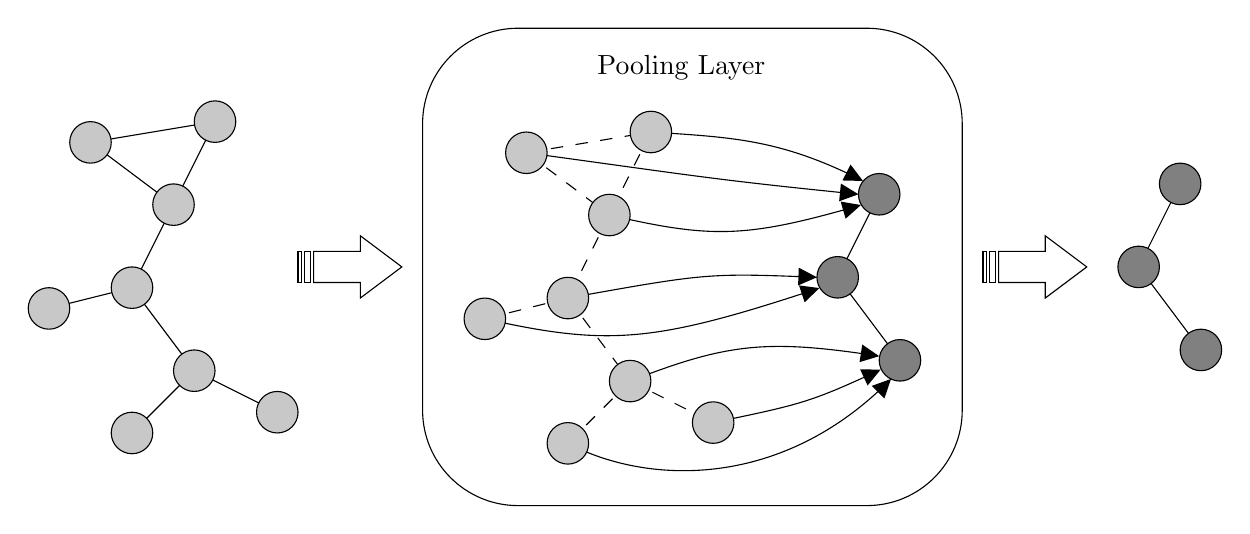
\begin{tikzpicture}[x=0.75pt,y=0.75pt,yscale=-1,xscale=1]
%uncomment if require: \path (0,300); %set diagram left start at 0, and has height of 300

%Straight Lines [id:da5096617344365821] 
\draw    (585,95) -- (565,135) ;
%Straight Lines [id:da9932827718765578] 
\draw    (565,135) -- (595,175) ;
%Curve Lines [id:da6905034262446312] 
\draw    (270,80) .. controls (352.62,91.31) and (359.81,92.89) .. (427.92,99.79) ;
\draw [shift={(430,100)}, rotate = 185.77] [fill={rgb, 255:red, 0; green, 0; blue, 0 }  ][line width=0.08]  [draw opacity=0] (8.93,-4.29) -- (0,0) -- (8.93,4.29) -- cycle    ;
%Curve Lines [id:da8335321724765272] 
\draw    (330,70) .. controls (368.17,72.52) and (391.5,73.29) .. (429.83,92.38) ;
\draw [shift={(432.2,93.58)}, rotate = 207] [fill={rgb, 255:red, 0; green, 0; blue, 0 }  ][line width=0.08]  [draw opacity=0] (8.93,-4.29) -- (0,0) -- (8.93,4.29) -- cycle    ;
%Curve Lines [id:da31100259312110135] 
\draw    (250,160) .. controls (309.35,173.29) and (331.51,171.46) .. (408.84,145.96) ;
\draw [shift={(411.2,145.18)}, rotate = 521.6700000000001] [fill={rgb, 255:red, 0; green, 0; blue, 0 }  ][line width=0.08]  [draw opacity=0] (8.93,-4.29) -- (0,0) -- (8.93,4.29) -- cycle    ;
%Curve Lines [id:da5677680537011585] 
\draw    (320,190) .. controls (366.25,171.95) and (385.37,169.74) .. (437.59,177.63) ;
\draw [shift={(440,178)}, rotate = 188.76] [fill={rgb, 255:red, 0; green, 0; blue, 0 }  ][line width=0.08]  [draw opacity=0] (8.93,-4.29) -- (0,0) -- (8.93,4.29) -- cycle    ;
%Curve Lines [id:da15435588971241] 
\draw    (360,210) .. controls (401.63,201.4) and (406.71,200.23) .. (438.22,185.63) ;
\draw [shift={(440.7,184.48)}, rotate = 515.05] [fill={rgb, 255:red, 0; green, 0; blue, 0 }  ][line width=0.08]  [draw opacity=0] (8.93,-4.29) -- (0,0) -- (8.93,4.29) -- cycle    ;
%Curve Lines [id:da7751491360366476] 
\draw    (290,220) .. controls (327.57,239.78) and (391.65,242.62) .. (444.11,190.57) ;
\draw [shift={(445.7,188.98)}, rotate = 494.49] [fill={rgb, 255:red, 0; green, 0; blue, 0 }  ][line width=0.08]  [draw opacity=0] (8.93,-4.29) -- (0,0) -- (8.93,4.29) -- cycle    ;
%Curve Lines [id:da9997311294079065] 
\draw    (310,110) .. controls (358.71,121.25) and (375.45,121.18) .. (428.74,105.88) ;
\draw [shift={(431.2,105.17)}, rotate = 523.85] [fill={rgb, 255:red, 0; green, 0; blue, 0 }  ][line width=0.08]  [draw opacity=0] (8.93,-4.29) -- (0,0) -- (8.93,4.29) -- cycle    ;
%Curve Lines [id:da5516088460235944] 
\draw    (290,150) .. controls (356.19,138.11) and (357.67,137.93) .. (407.68,139.91) ;
\draw [shift={(410,140)}, rotate = 182.27] [fill={rgb, 255:red, 0; green, 0; blue, 0 }  ][line width=0.08]  [draw opacity=0] (8.93,-4.29) -- (0,0) -- (8.93,4.29) -- cycle    ;
%Straight Lines [id:da42002527970780945] 
\draw    (60,75) -- (100,105) ;
%Straight Lines [id:da9625123729833738] 
\draw    (120,65) -- (100,105) ;
%Straight Lines [id:da011564512705323882] 
\draw    (60,75) -- (120,65) ;
%Straight Lines [id:da591791700605113] 
\draw    (100,105) -- (80,145) ;
%Straight Lines [id:da0520483680630226] 
\draw    (40,155) -- (80,145) ;
%Straight Lines [id:da243342242168614] 
\draw    (80,145) -- (110,185) ;
%Straight Lines [id:da29763945544745907] 
\draw    (110,185) -- (80,215) ;
%Straight Lines [id:da041191991130072436] 
\draw    (110,185) -- (150,205) ;
%Shape: Circle [id:dp7340107223648733] 
\draw  [fill={rgb, 255:red, 200; green, 200; blue, 200 }  ,fill opacity=1 ] (50,75) .. controls (50,69.48) and (54.48,65) .. (60,65) .. controls (65.52,65) and (70,69.48) .. (70,75) .. controls (70,80.52) and (65.52,85) .. (60,85) .. controls (54.48,85) and (50,80.52) .. (50,75) -- cycle ;
%Shape: Circle [id:dp00026389043378993726] 
\draw  [fill={rgb, 255:red, 200; green, 200; blue, 200 }  ,fill opacity=1 ] (110,65) .. controls (110,59.48) and (114.48,55) .. (120,55) .. controls (125.52,55) and (130,59.48) .. (130,65) .. controls (130,70.52) and (125.52,75) .. (120,75) .. controls (114.48,75) and (110,70.52) .. (110,65) -- cycle ;
%Shape: Circle [id:dp5553734560288552] 
\draw  [fill={rgb, 255:red, 200; green, 200; blue, 200 }  ,fill opacity=1 ] (90,105) .. controls (90,99.48) and (94.48,95) .. (100,95) .. controls (105.52,95) and (110,99.48) .. (110,105) .. controls (110,110.52) and (105.52,115) .. (100,115) .. controls (94.48,115) and (90,110.52) .. (90,105) -- cycle ;
%Shape: Circle [id:dp7685657012179221] 
\draw  [fill={rgb, 255:red, 200; green, 200; blue, 200 }  ,fill opacity=1 ] (70,145) .. controls (70,139.48) and (74.48,135) .. (80,135) .. controls (85.52,135) and (90,139.48) .. (90,145) .. controls (90,150.52) and (85.52,155) .. (80,155) .. controls (74.48,155) and (70,150.52) .. (70,145) -- cycle ;
%Shape: Circle [id:dp8225576337985958] 
\draw  [fill={rgb, 255:red, 200; green, 200; blue, 200 }  ,fill opacity=1 ] (30,155) .. controls (30,149.48) and (34.48,145) .. (40,145) .. controls (45.52,145) and (50,149.48) .. (50,155) .. controls (50,160.52) and (45.52,165) .. (40,165) .. controls (34.48,165) and (30,160.52) .. (30,155) -- cycle ;
%Shape: Circle [id:dp8048870433512154] 
\draw  [fill={rgb, 255:red, 200; green, 200; blue, 200 }  ,fill opacity=1 ] (100,185) .. controls (100,179.48) and (104.48,175) .. (110,175) .. controls (115.52,175) and (120,179.48) .. (120,185) .. controls (120,190.52) and (115.52,195) .. (110,195) .. controls (104.48,195) and (100,190.52) .. (100,185) -- cycle ;
%Shape: Circle [id:dp3899524469262352] 
\draw  [fill={rgb, 255:red, 200; green, 200; blue, 200 }  ,fill opacity=1 ] (70,215) .. controls (70,209.48) and (74.48,205) .. (80,205) .. controls (85.52,205) and (90,209.48) .. (90,215) .. controls (90,220.52) and (85.52,225) .. (80,225) .. controls (74.48,225) and (70,220.52) .. (70,215) -- cycle ;
%Shape: Circle [id:dp40591726527712235] 
\draw  [fill={rgb, 255:red, 200; green, 200; blue, 200 }  ,fill opacity=1 ] (140,205) .. controls (140,199.48) and (144.48,195) .. (150,195) .. controls (155.52,195) and (160,199.48) .. (160,205) .. controls (160,210.52) and (155.52,215) .. (150,215) .. controls (144.48,215) and (140,210.52) .. (140,205) -- cycle ;
%Straight Lines [id:da673763044302859] 
\draw  [dash pattern={on 4.5pt off 4.5pt}]  (270,80) -- (310,110) ;
%Straight Lines [id:da9124441607803917] 
\draw  [dash pattern={on 4.5pt off 4.5pt}]  (330,70) -- (310,110) ;
%Straight Lines [id:da03995998781592447] 
\draw  [dash pattern={on 4.5pt off 4.5pt}]  (270,80) -- (330,70) ;
%Straight Lines [id:da8129344208516425] 
\draw  [dash pattern={on 4.5pt off 4.5pt}]  (310,110) -- (290,150) ;
%Straight Lines [id:da6336124502461815] 
\draw  [dash pattern={on 4.5pt off 4.5pt}]  (250,160) -- (290,150) ;
%Straight Lines [id:da8022108969555355] 
\draw  [dash pattern={on 4.5pt off 4.5pt}]  (290,150) -- (320,190) ;
%Straight Lines [id:da3098627478952969] 
\draw  [dash pattern={on 4.5pt off 4.5pt}]  (320,190) -- (290,220) ;
%Straight Lines [id:da14837892723690072] 
\draw  [dash pattern={on 4.5pt off 4.5pt}]  (320,190) -- (360,210) ;
%Shape: Circle [id:dp42990613199323735] 
\draw  [fill={rgb, 255:red, 200; green, 200; blue, 200 }  ,fill opacity=1 ] (260,80) .. controls (260,74.48) and (264.48,70) .. (270,70) .. controls (275.52,70) and (280,74.48) .. (280,80) .. controls (280,85.52) and (275.52,90) .. (270,90) .. controls (264.48,90) and (260,85.52) .. (260,80) -- cycle ;
%Shape: Circle [id:dp2754617992158239] 
\draw  [fill={rgb, 255:red, 200; green, 200; blue, 200 }  ,fill opacity=1 ] (320,70) .. controls (320,64.48) and (324.48,60) .. (330,60) .. controls (335.52,60) and (340,64.48) .. (340,70) .. controls (340,75.52) and (335.52,80) .. (330,80) .. controls (324.48,80) and (320,75.52) .. (320,70) -- cycle ;
%Shape: Circle [id:dp21321858378283642] 
\draw  [fill={rgb, 255:red, 200; green, 200; blue, 200 }  ,fill opacity=1 ] (300,110) .. controls (300,104.48) and (304.48,100) .. (310,100) .. controls (315.52,100) and (320,104.48) .. (320,110) .. controls (320,115.52) and (315.52,120) .. (310,120) .. controls (304.48,120) and (300,115.52) .. (300,110) -- cycle ;
%Shape: Circle [id:dp5661953542799116] 
\draw  [fill={rgb, 255:red, 200; green, 200; blue, 200 }  ,fill opacity=1 ] (280,150) .. controls (280,144.48) and (284.48,140) .. (290,140) .. controls (295.52,140) and (300,144.48) .. (300,150) .. controls (300,155.52) and (295.52,160) .. (290,160) .. controls (284.48,160) and (280,155.52) .. (280,150) -- cycle ;
%Shape: Circle [id:dp5442339392428344] 
\draw  [fill={rgb, 255:red, 200; green, 200; blue, 200 }  ,fill opacity=1 ] (240,160) .. controls (240,154.48) and (244.48,150) .. (250,150) .. controls (255.52,150) and (260,154.48) .. (260,160) .. controls (260,165.52) and (255.52,170) .. (250,170) .. controls (244.48,170) and (240,165.52) .. (240,160) -- cycle ;
%Shape: Circle [id:dp00011290407505515354] 
\draw  [fill={rgb, 255:red, 200; green, 200; blue, 200 }  ,fill opacity=1 ] (310,190) .. controls (310,184.48) and (314.48,180) .. (320,180) .. controls (325.52,180) and (330,184.48) .. (330,190) .. controls (330,195.52) and (325.52,200) .. (320,200) .. controls (314.48,200) and (310,195.52) .. (310,190) -- cycle ;
%Shape: Circle [id:dp518700726149034] 
\draw  [fill={rgb, 255:red, 200; green, 200; blue, 200 }  ,fill opacity=1 ] (280,220) .. controls (280,214.48) and (284.48,210) .. (290,210) .. controls (295.52,210) and (300,214.48) .. (300,220) .. controls (300,225.52) and (295.52,230) .. (290,230) .. controls (284.48,230) and (280,225.52) .. (280,220) -- cycle ;
%Shape: Circle [id:dp5730004415356564] 
\draw  [fill={rgb, 255:red, 200; green, 200; blue, 200 }  ,fill opacity=1 ] (350,210) .. controls (350,204.48) and (354.48,200) .. (360,200) .. controls (365.52,200) and (370,204.48) .. (370,210) .. controls (370,215.52) and (365.52,220) .. (360,220) .. controls (354.48,220) and (350,215.52) .. (350,210) -- cycle ;
%Straight Lines [id:da001623419930635972] 
\draw    (440,100) -- (420,140) ;
%Straight Lines [id:da015699553757238416] 
\draw    (420,140) -- (450,180) ;
%Shape: Circle [id:dp36211696768410073] 
\draw  [fill={rgb, 255:red, 128; green, 128; blue, 128 }  ,fill opacity=1 ] (430,100) .. controls (430,94.48) and (434.48,90) .. (440,90) .. controls (445.52,90) and (450,94.48) .. (450,100) .. controls (450,105.52) and (445.52,110) .. (440,110) .. controls (434.48,110) and (430,105.52) .. (430,100) -- cycle ;
%Shape: Circle [id:dp01799126024681974] 
\draw  [fill={rgb, 255:red, 128; green, 128; blue, 128 }  ,fill opacity=1 ] (410,140) .. controls (410,134.48) and (414.48,130) .. (420,130) .. controls (425.52,130) and (430,134.48) .. (430,140) .. controls (430,145.52) and (425.52,150) .. (420,150) .. controls (414.48,150) and (410,145.52) .. (410,140) -- cycle ;
%Shape: Circle [id:dp058899920078356205] 
\draw  [fill={rgb, 255:red, 128; green, 128; blue, 128 }  ,fill opacity=1 ] (440,180) .. controls (440,174.48) and (444.48,170) .. (450,170) .. controls (455.52,170) and (460,174.48) .. (460,180) .. controls (460,185.52) and (455.52,190) .. (450,190) .. controls (444.48,190) and (440,185.52) .. (440,180) -- cycle ;
%Shape: Circle [id:dp5649766452502909] 
\draw  [fill={rgb, 255:red, 128; green, 128; blue, 128 }  ,fill opacity=1 ] (575,95) .. controls (575,89.48) and (579.48,85) .. (585,85) .. controls (590.52,85) and (595,89.48) .. (595,95) .. controls (595,100.52) and (590.52,105) .. (585,105) .. controls (579.48,105) and (575,100.52) .. (575,95) -- cycle ;
%Shape: Circle [id:dp5246365191278834] 
\draw  [fill={rgb, 255:red, 128; green, 128; blue, 128 }  ,fill opacity=1 ] (555,135) .. controls (555,129.48) and (559.48,125) .. (565,125) .. controls (570.52,125) and (575,129.48) .. (575,135) .. controls (575,140.52) and (570.52,145) .. (565,145) .. controls (559.48,145) and (555,140.52) .. (555,135) -- cycle ;
%Shape: Circle [id:dp5766159917435185] 
\draw  [fill={rgb, 255:red, 128; green, 128; blue, 128 }  ,fill opacity=1 ] (585,175) .. controls (585,169.48) and (589.48,165) .. (595,165) .. controls (600.52,165) and (605,169.48) .. (605,175) .. controls (605,180.52) and (600.52,185) .. (595,185) .. controls (589.48,185) and (585,180.52) .. (585,175) -- cycle ;
%Rounded Rect [id:dp6303563718720424] 
\draw   (220,66) .. controls (220,40.59) and (240.59,20) .. (266,20) -- (434,20) .. controls (459.41,20) and (480,40.59) .. (480,66) -- (480,204) .. controls (480,229.41) and (459.41,250) .. (434,250) -- (266,250) .. controls (240.59,250) and (220,229.41) .. (220,204) -- cycle ;
%Striped Right Arrow [id:dp8981402107639092] 
\draw   (167.5,127.5) -- (190,127.5) -- (190,120) -- (210,135) -- (190,150) -- (190,142.5) -- (167.5,142.5) -- cycle ;\draw   (160,127.5) -- (161.5,127.5) -- (161.5,142.5) -- (160,142.5) -- cycle ;\draw   (163,127.5) -- (166,127.5) -- (166,142.5) -- (163,142.5) -- cycle ;
%Striped Right Arrow [id:dp4519194983259933] 
\draw   (497.5,127.5) -- (520,127.5) -- (520,120) -- (540,135) -- (520,150) -- (520,142.5) -- (497.5,142.5) -- cycle ;\draw   (490,127.5) -- (491.5,127.5) -- (491.5,142.5) -- (490,142.5) -- cycle ;\draw   (493,127.5) -- (496,127.5) -- (496,142.5) -- (493,142.5) -- cycle ;

% Text Node
\draw (303,32) node [anchor=north west][inner sep=0.75pt]   [align=left] {Pooling Layer};


\end{tikzpicture}}
    \caption{A visual example of a graph pooling layer.}
    \label{fig:pooling}
\end{figure*}
Topological pooling, on the other hand,  uses not-differentiable methods which leverage the global structure of the graph, and the communities beneath it. These methods work by grouping nodes according to well known graph theory tools, such as spectral clustering (see \eg \citet{vonluxburg2007tutorialspectralclustering, dhillon2007weightedgraphcuts}).

\subsection{Regularization}
\glspl{dgn} are trained with regular losses, such as \gls{ce} for classification and \gls{mse} for regression. Besides standard regularization techniques, the objective function is often regularized through unsupervised loss functions, which impose priors on which kinds of
structures the network should preferably learn. The regularized objective function for supervised tasks\footnote{We use a generic target $y$ to imply that this formulation is task-independent.} has the form:
$$\argmin_{\Param} \Loss(\Param, (\Vector{x}_{\Graph{g}}, y)) + \lambda \sum_{\ell=1}^L \Psi(\LayerStateMat{g}{\ell}),$$
were $\Psi$ is a regularization function weighted by a regularization coefficient $\lambda$, that is applied at each layer $\ell$ to the set of hidden states of the nodes, represented as a matrix $\Matrix{h}_{{\Graph{g}}}^{(\ell)} \in \Real^{n \times h}$. An example of regularization widely employed in practical settings is the \emph{link prediction} unsupervised loss, defined as:
\begin{align}
    \Psi(\LayerStateMat{g}{\ell}) = \sum_{u,v} \Norm{\StateVector{v}{\ell} - \StateVector{u}{\ell}}_2,
\end{align}
where the summation ranges over all possible combinations of nodes. Basically, when this loss is minimized, it biases the network towards producing node representations that are more similar for nodes connected by an edge. Notably, this loss can be also used in isolation to tackle link prediction tasks, \ie tasks where the downstream network must predict unseen links between the nodes.

\section{The Evaluation of Deep Graph Networks}
Over the years, \glspl{dgn} have yielded strong performances on several predictive tasks, becoming the \defacto learning tool for graph-related problems. Given their appeal, several \gls{dgn} architectures have been developed recently. These architectures require a thorough evaluation to understand which one is better suited for a certain task. The evaluation requires both an extensive model selection phase, to select appropriate hyper-parameters, as well as a model evaluation phase to obtain an estimation of the generalization ability of the network. In the literature, the evaluation of \glspl{dgn} is carried out on a variety of benchmark datasets, generally from the chemistry and social sciences domains, where graphs are used to represent molecules and social networks, respectively. However, as pointed out by researchers \citep{lipton2018troubling}, the papers that introduce novel architectures often adopt not reproducible or unfair experimental setups, which make the comparisons among models unreliable. In this section, we present three contributions related to address this important issue. Specifically, we:
\begin{itemize}
    \item provide a rigorous evaluation of existing \glspl{dgn} models in the context of graph classification, using a standardized and reproducible experimental environment. Specifically, we perform a large number of experiments within a rigorous model selection and assessment framework, in which all models are compared using the same node features and data splits;
    \item investigate if and to what extent current \gls{dgn} models can effectively exploit graph structure on the evaluation benchmarks. To this end, we also evaluate two domain-specific structure-agnostic baselines, whose purpose is to disentangle the contribution of structural information from node features;
    \item study the effect of node degrees as features in social datasets. We show that adding node degrees to the node features can be beneficial, and it has implications as to how many convolutional layers are needed to obtain good performances.
\end{itemize}

\subsection{Datasets}
All  graph  datasets  are  publicly  available \citep{kersting2016benchmark}  and  represent  a  relevant subset of those most frequently used in literature to compare \glspl{dgn}. Some collect molecular graphs, while others contain social graphs. Specifically, we use the following chemical datasets:
\begin{itemize}
    \item D\&D \citep{dobson2003dd} is a graph dataset in which nodes are amino acids, and there is an edge between two nodes if they are they are neighbors in the amino-acid sequence or in 3D space. The task is a binary classification one, where the objective is to determine whether a graph represents an enzyme or non-enzyme;
    \item PROTEINS \citep{borgwardt2005proteins} is a subset of D\&D where the largest graphs have been removed;
    \item NCI1 \citep{wale2008nci1} is a dataset made of chemical compounds screened for ability to suppress or inhibit the growth of a panel of human tumor cell lines. The task is a binary classification one, where the objective is to determine if a chemical compound acts as suppressor or inhibitor;
    \item ENZYMES is a dataset of enzymes taken from the BRENDA enzyme database \citep{schomburg2004enzymes}. In this case, the task is to correctly assign each enzyme to one out of 6 Enzyme Commission (EC) numbers.
\end{itemize}
As regards datasets containing social graphs, we use the following:
\begin{itemize}
    \item IMDB-BINARY and IMDB-MULTI \citep{yanardag2015imdbredditcollab} are movie collaboration datasets. Each graph is an ego-network where nodes are actors or actresses, and edges connect two actors/actresses which star in the same movie. Each graph has been extracted from a pre-specified genre of movies, and the task is to classify the genre graph the ego-network is derived from.
    \item REDDIT-5K \citep{yanardag2015imdbredditcollab} is a dataset where each graph represents an online thread on the Reddit platform, and nodes correspond to users. Two nodes are connected by an edge if at least one of the two users commented each other on the thread. The task is to classify each graph to a corresponding community (a sub-reddit);
    \item COLLAB \citep{yanardag2015imdbredditcollab} is a dataset where each graph is an ego-network of different researchers from some research field. There is an edge between two authors if they coauthored a scientific article. The task is to classify each ego-network to the corresponding field of research.
\end{itemize}
All node features are discrete (we shall refer to them as node labels equivalently). The only exception is the ENZYMES dataset, which also has an additional 18 continuous features. The social datasets do not have node features. In this case, we use either an uninformative label for all nodes, or the node degree. Specifically, social datasets are used to understand whether the models are able to learn structural features on their own or not. The statistics of the datasets, which include number of graphs, number of target classes, average number of nodes per graph, average number of nodes per graph, and number of node labels (if any) are reported in Table \ref{tab:comparison-datasets}.
\begin{table}[h!]
    \footnotesize
    \renewcommand\arraystretch{1.1}
    \caption{Dataset Statistics. Note that, when node labels are not present, we either assign the same feature or the degree to all the nodes in the dataset.} \label{tab:comparison-datasets}
    \begin{center}
    \begin{tabular}{c l c c c c c}
    \toprule
    &  & \Thead{Graphs} & \Thead{Classes} & \Thead{Avg. Nodes} & \Thead{Avg. Edges} & \Thead{Labels}\\
    \toprule
    \multirow{4}{*}{\rotatebox[origin=c]{90}{\Thead{\textsc{Chem.}}}}
    &D\&D            & 1178 & 2 & 284.32 & 715.66 & 89 \\
    &ENZYMES       &  600 & 6 &  32.63 &  64.14 &  3 \\
    &NCI1          & 4110 & 2 &  29.87 &  32.30 & 37 \\
    &PROTEINS      & 1113 & 2 &  39.06 &  72.82 &  3 \\
    \midrule
    \multirow{5}{*}{\rotatebox[origin=c]{90}{\Thead{\textsc{Social}}}}
    &COLLAB     & 5000 & 3 & 74.49 & 2457.78 &  - \\
    &IMDB-BINARY   & 1000 & 2 &  19.77 &  96.53 &  - \\
    &IMDB-MULTI    & 1500 & 3 &  13.00 &  65.94 &  - \\
    &REDDIT-BINARY & 2000 & 2 & 429.63 & 497.75 &  - \\
    &REDDIT-5K     & 4999 & 5 & 508.82 & 594.87 &  - \\
    \bottomrule
    \end{tabular}
    \end{center}
\end{table}

\subsection{Architectures}\label{sec:comparison-architectures}
In total, we choose five different \gls{dgn} architectures. The high-level structure of the \gls{dgn} comprises an input layer, a stack of one or more \glspl{gcl}, a readout layer and a final MLP classifier, which maps the graph embedding to the dataset-dependent output. Following, we describe in detail the kinds of \gls{gcl} used by the \glspl{dgn}, and the specific hyper-parameters optimized for each of them.

\paragraph{Graph Isomorphism Network} The \gls{gin} convolutional layer by \cite{xu2019gin} is implemented as follows:
$$\StateVector{v}{\ell} = \Fun{MLP} \Par{(1 + \epsilon^{(\ell)})\,\Elem{h}{v}^{(\ell-1)} + \sum_{u \in \Neigh(v)} \StateVector{u}{\ell-1}},$$
where $\epsilon \in \Real$ is a trainable parameter, and MLP is a neural network with 2 hidden layers, each one consisting of a linear transformation, followed by a BatchNorm layer and a \gls{relu} non-linearity. The first layer of the \gls{dgn} is not a \gls{gcl}, but a graph readout that sums the node features, and passes them through an MLP identical to the one just described. The graph embedding obtained by this layer is then summed to the graph embeddings computed by the \glspl{gcl}. For this architecture, we choose the following hyper-parameters: number of layers, size of the hidden state at each layer, and type of readout function (for the first non-convolutional layer as well).

\paragraph{GraphSAGE}
The Graph SAmple and aggreGatE (GraphSAGE) layer by \cite{hamilton2017graphsage} is implemented as follows:
$$\StateVector{v}{\ell} = \sigma\Par{\LayerMatrix{w}{\ell}\StateVector{u}{\ell-1} + \frac{1}{|\Neigh(v)|} \LayerMatrix{U}{\ell} \sum_{u \in \Neigh(v)} \StateVector{u}{\ell-1}}.$$
Notice that the original formulation also implements a form of node sampling, since it is applied to large graphs. Here, since the size of the graph we deal with is manageable, we do not implement node sampling.

\paragraph{GraphSAGE + DiffPool}
In order to have a representative \gls{dgn} with pooling, we tested a variant of GraphSAGE, where a DiffPool layer is added to the network after every GraphSAGE convolution. Internally, the DiffPool layer is implemented as in Section \ref{sec:pooling}, where $\Fun{DGN}_e$ and $\Fun{DGN}_p$ are a stack of 3 GraphSAGE layers respectively. Thus, one DiffPool layer requires to compute 6 graph convolutions. The number of clusters $k$ is deterministic, and is obtained as $\alpha M$, where $M$ is the maximum number of nodes among the graphs in the dataset, and $\alpha$ is a coarsening factor which is 0.1 if only one DiffPool layer is applied, and 0.25 otherwise.

\paragraph{ECC}
The Edge-Conditioned Convolutional layer by \cite{simonovsky2017ecc} is implemented as follows:
$$\StateVector{v}{\ell} = \sigma\Par{ \frac{1}{|\Neigh(v)|}\sum_{u \in \Neigh(v)} \Fun{MLP}(\Elem{e}{u,v})^{\Transpose} \StateVector{u}{\ell-1}},$$
where MLP is a neural network that computes a weight between the hidden state of the current node $\Elem{h}{v}^{(\ell-1)}$ and its generic neighbor $\StateVector{u}{\ell-1}$, using the edge feature vector as input, composed of one hidden layer with ReLU non-linearities and a subsequent linear output layer. Each convolutional layer of the corresponding \gls{dgn} is composed of a stack of three ECC layers.

\paragraph{DGCNN}
The graph convolutional layer of the Deep Graph Convolutional Neural Network (DGCNN) \citep{zhang2018dgcnn}, is the following:
$$\StateVector{v}{\ell} = \Fun{tanh} \Par{\LayerMatrix{w}{\ell} \sum_{u \in \Neigh(v)} \Matrix{D}^{-1}_{vu}\StateVector{u}{\ell-1}},$$
where $\Matrix{D}^{-1}$ is the inverse degree matrix. After all the convolutional layers are applied, the computation is followed by SortPool layer, which performs graph pooling, and a final 1-D \gls{cnn}.

\subsection{Baselines}
We compare the proposed architectures with two structure-agnostic baselines, one for molecular graphs, and one for social graphs. For molecular graphs, with the exception of graphs in the ENZYMES dataset, we use an \gls{mlp}-based model \citep{ralaivola2005graphkernels}, applied as follows to a generic graph $\GraphU{g}$:
$$\GraphRepr{g} = \Fun{MLP}\Par{\sum_{v \in \Nodes{g}} \Elem{x}{v}}.$$
This architecture corresponds to summing the node features together (which are one-hot encoded vectors representing the atom types), and applying an \gls{mlp} with 2 hidden layers with \gls{relu} non-linearities on top of them. In practice, the network counts the atom occurrences for each atom type, and computes non-linear transformation of this sum. Notice that the graph connectivity is not taken into account by the model.
For the social graphs, and for the graphs in the ENZYMES dataset (which uses 18 additional node features with respect to the other molecular datasets), we use the following architecture, applied to a generic graph $\GraphU{g}$ as follows:
$$\GraphRepr{g} = \Fun{MLP}_2\Par{\sum_{v \in \Nodes{g}} \Fun{MLP}_1(\Elem{x}{v})},$$
where $\Fun{MLP}_1$ is a linear layer plus a \gls{relu} non-linearity, and $\Fun{MLP}_2$ is a two hidden layer \gls{mlp} with \gls{relu} non linearities \citep{zaheer2017deepsets}. Notice that even in this case we do not take into account the graph connectivity. The role of these baselines is to provide feedback on the effectiveness of \glspl{dgn} on a specific dataset. Specifically, if a \gls{dgn} performs similarly to a structure-agnostic baseline, one can draw two possible conclusions: either the task does not need structural information to be effectively solved, or the \gls{dgn} is not exploiting graph structure adequately. While the former can be verified through domain-specific human expertise, the second is more difficult to assess, as multiple factors come into play such as the size of the training dataset, the structural inductive bias imposed by the architecture and the selected hyper-parameters. Nevertheless, a significant improvement with respect to a baseline is a strong indicator that graph structure has been exploited.

\subsection{Experimental Setup}\label{sec:comparison-exp-setup}
In all our experiments, we use classification accuracy (\ie the percentage of correctly classified graphs out of the total number of predictions) as performance metric.
Our evaluation pipeline consists in an outer $10$-fold CV for model assessment, and an inner holdout technique with a 90\%/10\% training/validation split for model selection. After \emph{each} model selection, we train the winning model three times on the whole training fold, holding out a random fraction (10\%) of the data to perform early stopping. We do this in order to contrast the effect of unfavorable random weight initialization on test performances. The final score for each test fold is obtained as the average of these three runs. Importantly, all data splits have been precomputed, so that models are selected and evaluated on the same data partitions; this guarantees consistency in the evaluation. For the same reason, we also stratify all the class labels, so that the classes proportions are preserved inside each $10$-fold split, as well as in the internal holdout splits. With respect to the general \gls{dgn} architecture, we optimize learning rate and early stopping patience for every considered \gls{dgn}. All models are trained with the Adam \citep{kingma2015adam} optimizer with learning rate decay.

\paragraph{Hyper-Parameters}
For all the \gls{dgn} architectures, we tune the size of the hidden state of the convolutional layers and the number of layers. We keep the number of configurations roughly equal across all the tested models. The baselines are composed of a single layer, hence we only tune the hidden size. Besides architecture-specific hyper-parameters, we also tune others that are shared across all models, related to the training procedure. Specifically, for each model under evaluation, we optimize learning rate and learning rate decay. For GIN, we also optimize batch size. For the two baselines, we also optimize the L2 regularization factor. To be consistent with the literature, we implement early stopping with patience, where training stops if a number epochs have passed without improvement on the validation set. A high patience can favor model selection by making it less sensitive to fluctuations in the validation score at the cost of additional computation. The patience hyper-parameter is optimized for all the considered models. A table showing the complete grid of hyper-parameters we used for each \gls{dgn} under evaluation is reported in Appendix \ref{AppendixA}.

\paragraph{Computational Considerations}
The experiments required an extensive computational effort. For all models, the sizes of the hyper-parameter grids range from 32 to 72 possible configurations, depending on the number of hyper-parameters to choose from. The total number of single training runs to complete model assessment exceeds 47000. Such a large number requires an extensive use of parallelism, both in CPU and GPU, to conduct the experiments in a reasonable amount of time. In some cases (e.g. ECC in social datasets), training on a \emph{single} hyper-parameter configuration required more than 72 hours; consequently, the sequential exploration of one single grid would last months. For this reason, we limit the time to complete a single training to 72 hours.

\subsection{Results}
The experimental results are reported in Table \ref{tab:comparison-results-molecules} (for the chemical datasets) and Table \ref{tab:comparison-results-social} (for the social datasets). We notice an interesting trend on the D\&D, PROTEINS and ENZYMES datasets, where none of the \glspl{dgn} are able to improve over the baseline. Conversely, on the NCI1 dataset, the baseline is clearly outperformed: this result suggests that on this dataset, these \glspl{dgn} architectures are suited to exploit the structural information of the training graphs. This result is reinforced from empirical evidence: in fact, we observed in preliminary trials (not reported here) that an overly-parameterized baseline with 10000 hidden units and no regularization is not able to overfit the NCI1 training data completely, reaching around 67\% training accuracy, while a model such as GIN can easily overfit ($\approx 100\%$ accuracy) the training data. This indicates that, at least for the NCI1 dataset, the structural information hugely affects the ability to fit the training set. On social datasets, GIN seems to be the most performant model, reaching the best accuracy in three out of five datasets. However, in both chemical and social scenarios, the standard deviations are so large that all judgements about which model is better are speculative. Following, we summarize other relevant findings of our study.

\begin{table}[h!]
\renewcommand{\arraystretch}{1.1}
\centering
\caption{Results on chemical datasets with mean accuracy and standard deviation are reported. Best performances are highlighted in bold.}
\label{tab:comparison-results-molecules}
\begin{tabular}{l c c c c c}
\toprule
     & \textbf{D\&D} & \textbf{NCI1} & \textbf{PROTEINS} & \textbf{ENZYMES}\\
\midrule
 Baseline & $\mathbf{78.4}\pm 4.5 $ &  $69.8 \pm 2.2 $ &  $\mathbf{75.8} \pm 3.7 $ &  $\mathbf{65.2}\pm 6.4 $ \\
 DGCNN & $76.6 \pm 4.3 $ &  $76.4 \pm 1.7 $ &  $72.9 \pm 3.5 $ &  $38.9 \pm 5.7 $   \\
 DiffPool & $75.0 \pm 3.5 $ &  $76.9 \pm 1.9 $ &  $73.7 \pm 3.5 $ &  $59.5 \pm 5.6 $   \\
 ECC & $72.6 \pm 4.1 $ &  $76.2 \pm 1.4 $ &  $72.3 \pm 3.4 $ &  $29.5 \pm 8.2 $   \\
 GIN & $75.3 \pm 2.9 $ &  $\mathbf{80.0} \pm 1.4 $ &  $73.3 \pm 4.0 $ &  $59.6 \pm 4.5 $   \\
 GraphSAGE & $72.9 \pm 2.0 $ &  $76.0 \pm 1.8 $ &  $73.0 \pm 4.5 $ &  $58.2 \pm 6.0 $   \\
\bottomrule
\end{tabular}
\end{table}

\paragraph{The Importance of Baselines}
Our results confirm that structure-agnostic baselines are an essential tool to evaluate \glspl{dgn} under a clear perspective, as well as to extract useful insights on whether structure has been exploited. As an example, consider how none of the \glspl{dgn} surpasses the baseline on D\&D, PROTEINS and ENZYMES; based on this result, we argue that the state-of-the-art \glspl{dgn} we analyzed are not able to fully exploit the structure on such datasets yet. This contrasts with the current literature of chemistry, where structural properties of the molecular graph are strongly believed to correlate with molecular properties \citep{vanrossum1965chemical}. For this reason, we suggest not to over-emphasize small performance gains on these datasets. Currently, it is more likely that small fluctuations in performances are likely to be caused by other factors, such as random initializations, rather than a successful exploitation of the structure. In conclusion, we warmly recommend \gls{dgn} practitioners to include baseline comparisons in future works, in order to better characterize the extent of their contributions.

\begin{table}[h!]
\scriptsize
\renewcommand{\arraystretch}{1.1}
%\setlength{\tabcolsep}{10pt}
\centering
\caption{Results on social datasets with mean accuracy and standard deviation are reported. Best performances are highlighted in bold. OOR means Out of Resources, either time ($>$ 72 hours for a single training) or GPU memory. }
\label{tab:social-results}
\begin{tabular}{llccccc}
\toprule
     & & \textbf{IMDB-B} & \textbf{IMDB-M} & \textbf{REDDIT-B} & \textbf{REDDIT-5K} & \textbf{COLLAB}\\
    \midrule
\multirow{6}{*}{\rotatebox[origin=c]{90}{\textsc{No Features}}}
& Baseline & $50.7 \pm 2.4 $ &  $36.1 \pm 3.0 $ &  $72.1 \pm 7.8 $ &  $35.1 \pm 1.4 $ &  $55.0 \pm 1.9 $   \\
& DGCNN & $53.3 \pm 5.0 $ &  $38.6 \pm 2.2 $ &  $77.1 \pm 2.9 $ &  $35.7 \pm 1.8 $ &  $57.4 \pm 1.9 $   \\
& DiffPool & $68.3 \pm 6.1 $ &  $45.1 \pm 3.2 $ &  $76.6 \pm 2.4 $ &  $34.6 \pm 2.0 $ &  $67.7 \pm 1.9 $   \\
& ECC & $67.8 \pm 4.8 $ &  $44.8 \pm 3.1 $ &   OOR &   OOR &   OOR   \\
& GIN & $66.8 \pm 3.9 $ &  $42.2 \pm 4.6 $ &  $\mathbf{87.0} \pm 4.4 $ &  $\mathbf{53.8} \pm 5.9 $ &  $\mathbf{75.9} \pm 1.9 $   \\
& GraphSAGE & $\mathbf{69.9}\pm 4.6 $ &  $\mathbf{47.2}\pm 3.6 $ &  $86.1 \pm 2.0 $ &  $49.9 \pm 1.7 $ &  $71.6 \pm 1.5 $   \\

\midrule
\multirow{6}{*}{\rotatebox[origin=c]{90}{\textsc{With Degree}}}
& Baseline & $70.8 \pm 5.0 $ &  $\mathbf{49.1} \pm 3.5 $ &  $82.2 \pm 3.0 $ &  $52.2 \pm 1.5 $ &  $70.2 \pm 1.5 $   \\
& DGCNN & $69.2 \pm 3.0 $ &  $45.6 \pm 3.4 $ &  $87.8 \pm 2.5 $ &  $49.2 \pm 1.2 $ &  $71.2 \pm 1.9 $   \\
& DiffPool & $68.4 \pm 3.3 $ &  $45.6 \pm 3.4 $ &  $89.1 \pm 1.6 $ &  $53.8 \pm 1.4 $ &  $68.9 \pm 2.0 $   \\
& ECC & $67.7 \pm 2.8 $ &  $43.5 \pm 3.1 $ &   OOR &   OOR &   OOR   \\
& GIN & $\mathbf{71.2} \pm 3.9 $ &  $48.5 \pm 3.3 $ &  $\mathbf{89.9} \pm 1.9 $ &  $\mathbf{56.1} \pm 1.7 $ &  $\mathbf{75.6} \pm 2.3 $   \\
& GraphSAGE & $68.8 \pm 4.5 $ &  $47.6 \pm 3.5 $ &  $84.3 \pm 1.9 $ &  $50.0 \pm 1.3 $ &  $73.9 \pm 1.7 $   \\
\bottomrule
\end{tabular}
\label{tab:comparison-results-social}
\end{table}


\paragraph{The Effect of Node Degree}
Based on our results, adding the node degree to the input features almost always results in a performance improvement, sometimes very strong, on social datasets. For example, adding the degree information to the baseline improves performances of $\approx 15$\% across all datasets, up to being competitive with the examined \glspl{dgn}. In particular, the baseline achieves the best performance on IMDB-MULTI, and performs very close to the best model (GIN) on IMDB-BINARY. In contrast, the addition of degree information is less impacting for most \glspl{dgn}. This result is somewhat expected, since they are supposed to automatically extract the degree information from the structure. One notable exception to this trend is DGCNN, which explicitly needs the addition of node degrees to perform well across all datasets. We observe that the ranking of the models, after the addition of the degrees, drastically changes; this raises the question about the impact of other structural features (such as clustering coefficient) on performances, which we leave to future works. In a further experiment, we reason about whether the degree has an influence on the number of layers that are necessary to solve the task. We investigate the matter by computing the median number of layers of the winning model in each of the 10 different folds. These results are shown in Table \ref{tab:effect-of-degree}. Given the benefit given by the addition of the node degree feature, we hypothesize that models such as DGCNN learn features correlated to the node degrees in the very first layers; this learned information helps to perform well in the tasks using fewer convolutional layers.

\begin{table}[h!]

\footnotesize
\renewcommand\arraystretch{1.1}
\caption{The table displays the median number of selcted layers in relation to the addition of node degrees as input features on all social datasets. 1 indicates that an uninformative feature is used as node label.}
\begin{center}
\begin{tabular}{lcccccccccc}
\cmidrule{2-11}
          & \multicolumn{2}{c}{\textbf{IMDB-B}} & \multicolumn{2}{c}{\textbf{IMDB-M}} & \multicolumn{2}{c}{\textbf{REDDIT-B}} & \multicolumn{2}{c}{\textbf{REDDIT-M}} & \multicolumn{2}{c}{\textbf{COLLAB}} \\
          \cmidrule(lr){2-3}\cmidrule(lr){4-5}\cmidrule(lr){6-7}\cmidrule(lr){8-9}\cmidrule(lr){10-11}
          & \textbf{1}           & \textbf{DEG} & \textbf{1}           & \textbf{DEG} & \textbf{1}           & \textbf{DEG} & \textbf{1}           & \textbf{DEG} & \textbf{1}           & \textbf{DEG}          \\
          \midrule
DGCNN     & 3           & 3            & 3.5          & 3           & 4          & 3            & 3          & 2            & 4           & 2            \\
DiffPool  & 1           & 2            & 2            & 1           & 2          & 2            & 2          & 1            & 2           & 1.5          \\
ECC       & 1           & 2            & 1            & 1           & -          & -            & -          & -            & -           & -            \\
GIN       & 3           & 2            & 4            & 2           & 4          & 4            & 4          & 3            & 4           & 4            \\
GraphSAGE & 4           & 3            & 5            & 4           & 3          & 4            & 3          & 5            & 3           & 5\\           
\bottomrule
\end{tabular}
\end{center}
\label{tab:effect-of-degree}
\end{table}

\paragraph{Comparison with Published Results}
Figure \ref{fig:comparison-plot} compares the average values of our test results (shown with a square marker) to those reported in the literature (shown with a triangle marker). In addition, we plot the average of our validation results across the 10 different model selections (shown with a circle marker). From the plot, it is clear that our results are in most cases different from published results, and the gap between the two estimates is usually consistent. Moreover, and differently from results in the literature, our average validation accuracies are consistently similar to the test accuracies, which indicates that our estimates are less biased in general. We emphasize that our results are \emph{i}) obtained within the rigorous model selection and evaluation framework; \emph{ii}) fair in terms of how the data was split, and which features have been used for all competitors; \emph{iii}) reproducible\footnote{Code, hyper-parameters and data splits are available at \url{https://github.com/diningphil/gnn-comparison}}.

\begin{figure}[h!]
    \centering
    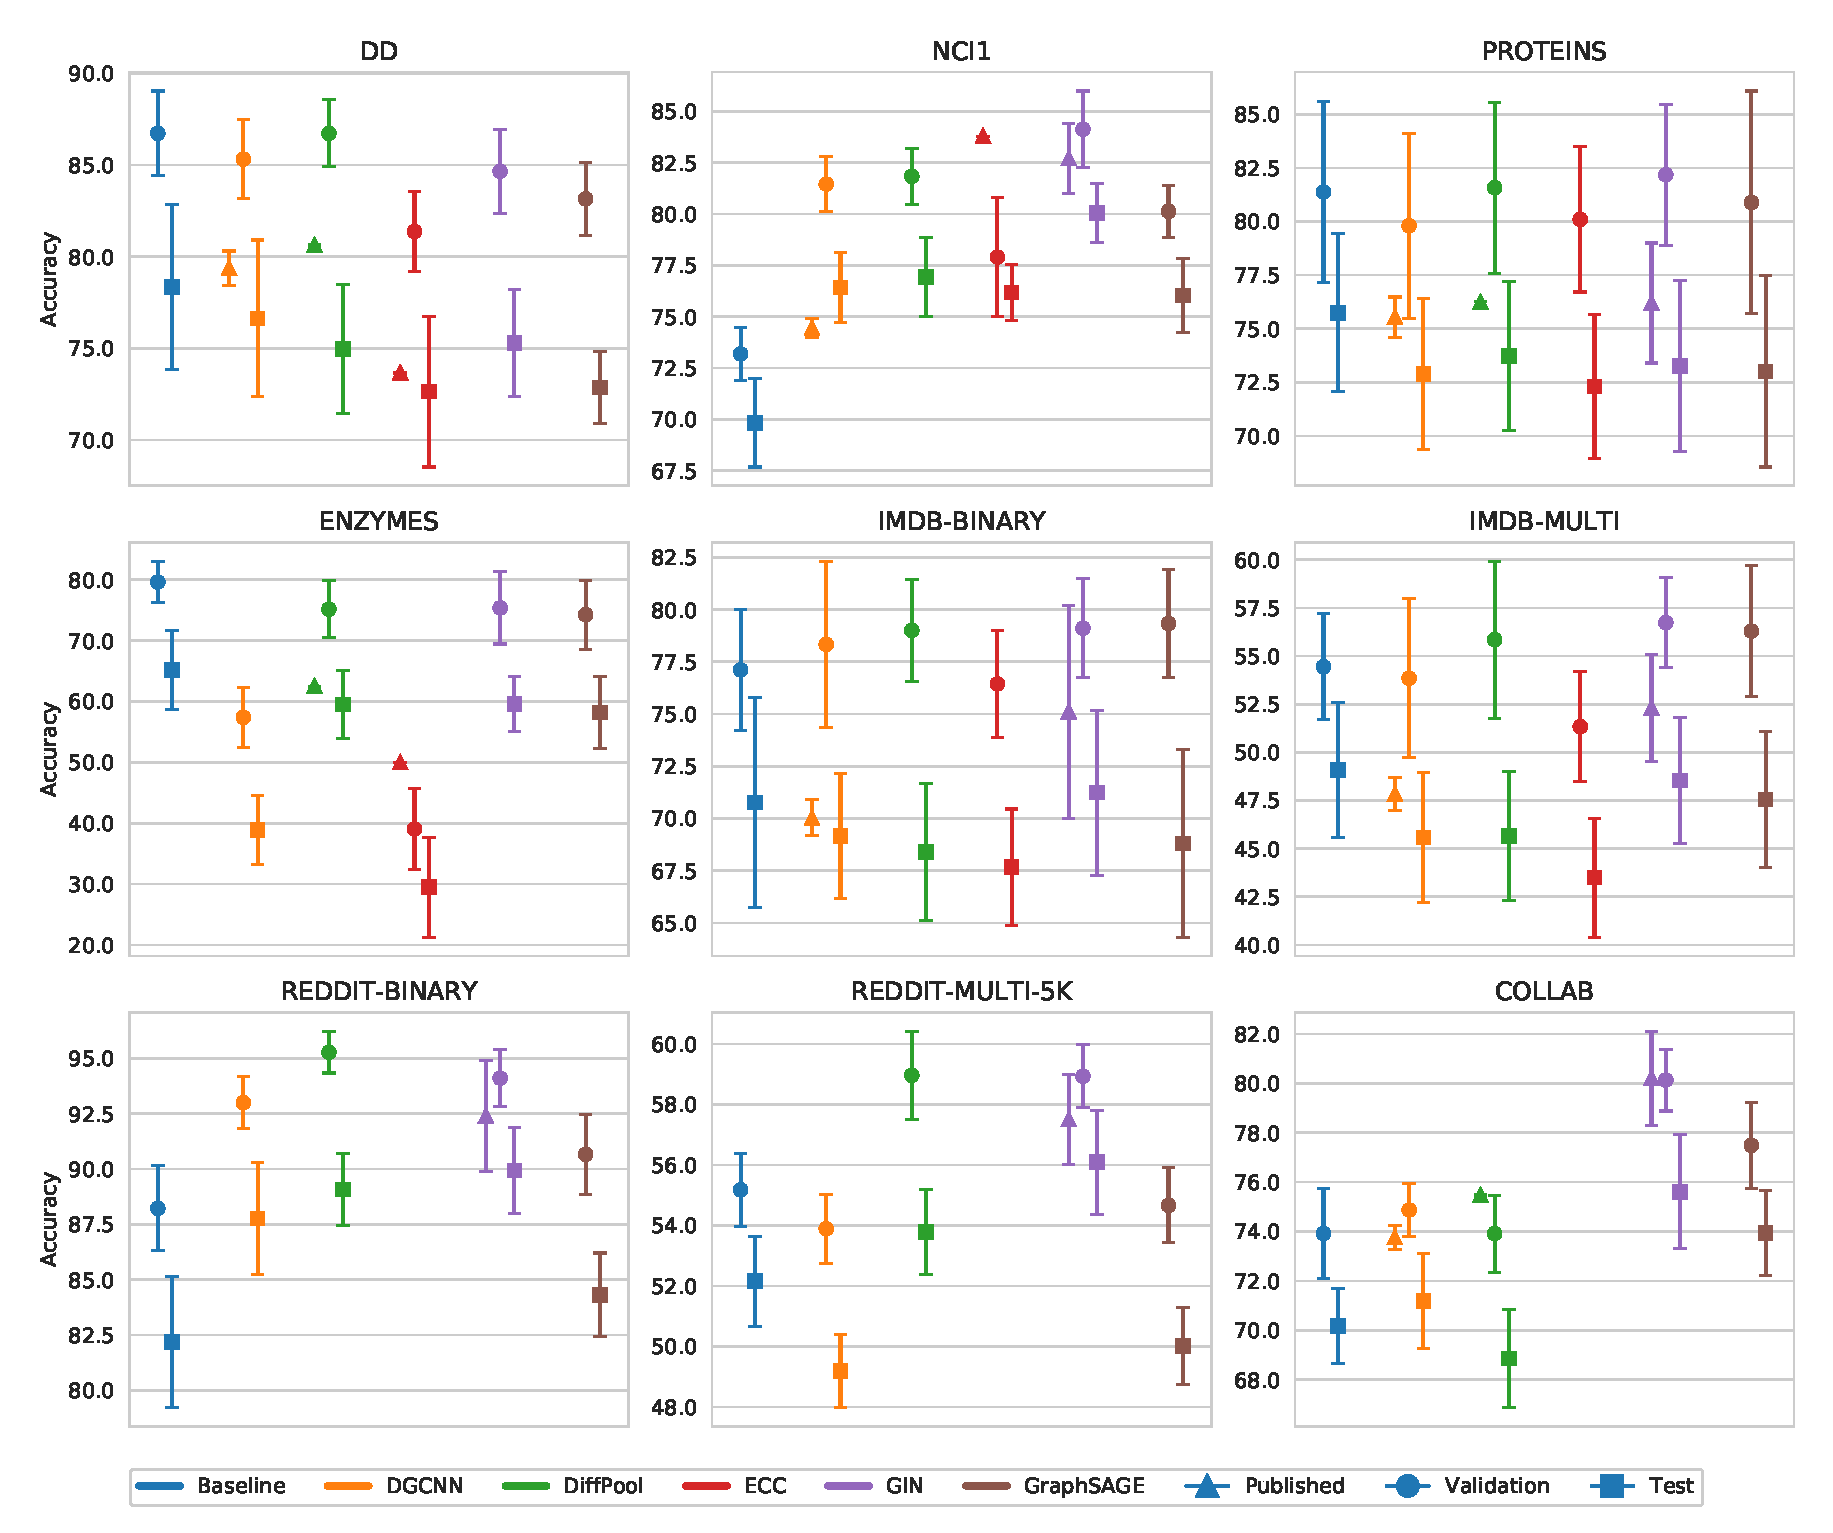
\includegraphics[width=\linewidth]{Figures/Chapter4/07-comparison-results.eps}
    \caption{Results.}
    \label{fig:comparison-plot}
\end{figure}

\subsection{Conclusions}
In this section, we showed how a rigorous empirical evaluation of \glspl{dgn} can help to design better experiments, and to draw more informed conclusions as regards the potential impact of novel architectures. This has been possible by introducing a clear and reproducible environment for benchmarking current and future \gls{dgn} architectures, as well as with reliable and reproducible results to which \gls{dgn} practitioners can test novel architectures. This work will hopefully prove useful to researchers and practitioners that want to compare \glspl{dgn} in a more rigorous way.
